% --------------------------
% ANÁLISIS DEL CONJUNTO DE DATOS DEPURADO
% --------------------------
\section{Análisis del conjunto de datos}
\label{sec:analisis_conjunto_datos}

En esta sección se presenta un análisis detallado del conjunto de datos, que incluye la identificación de patrones y tendencias en las trayectorias individuales. El conjunto de datos contiene puntos de recorrido obtenidos a lo largo de diez días. Por lo que el primer acercamiento del análisis es poder ver la distribución de los puntos de recorrido en cada día registrado por medio un histrograma por día. Para crear estos historgramas se ejecuta el código del Apéndice \ref{cod:identifier_histogram_daily}. A continuación, se muestran estos histogramas.

\begin{figure}[htbp]
    \centering
    \begin{subfigure}[t]{0.48\textwidth-1em}
        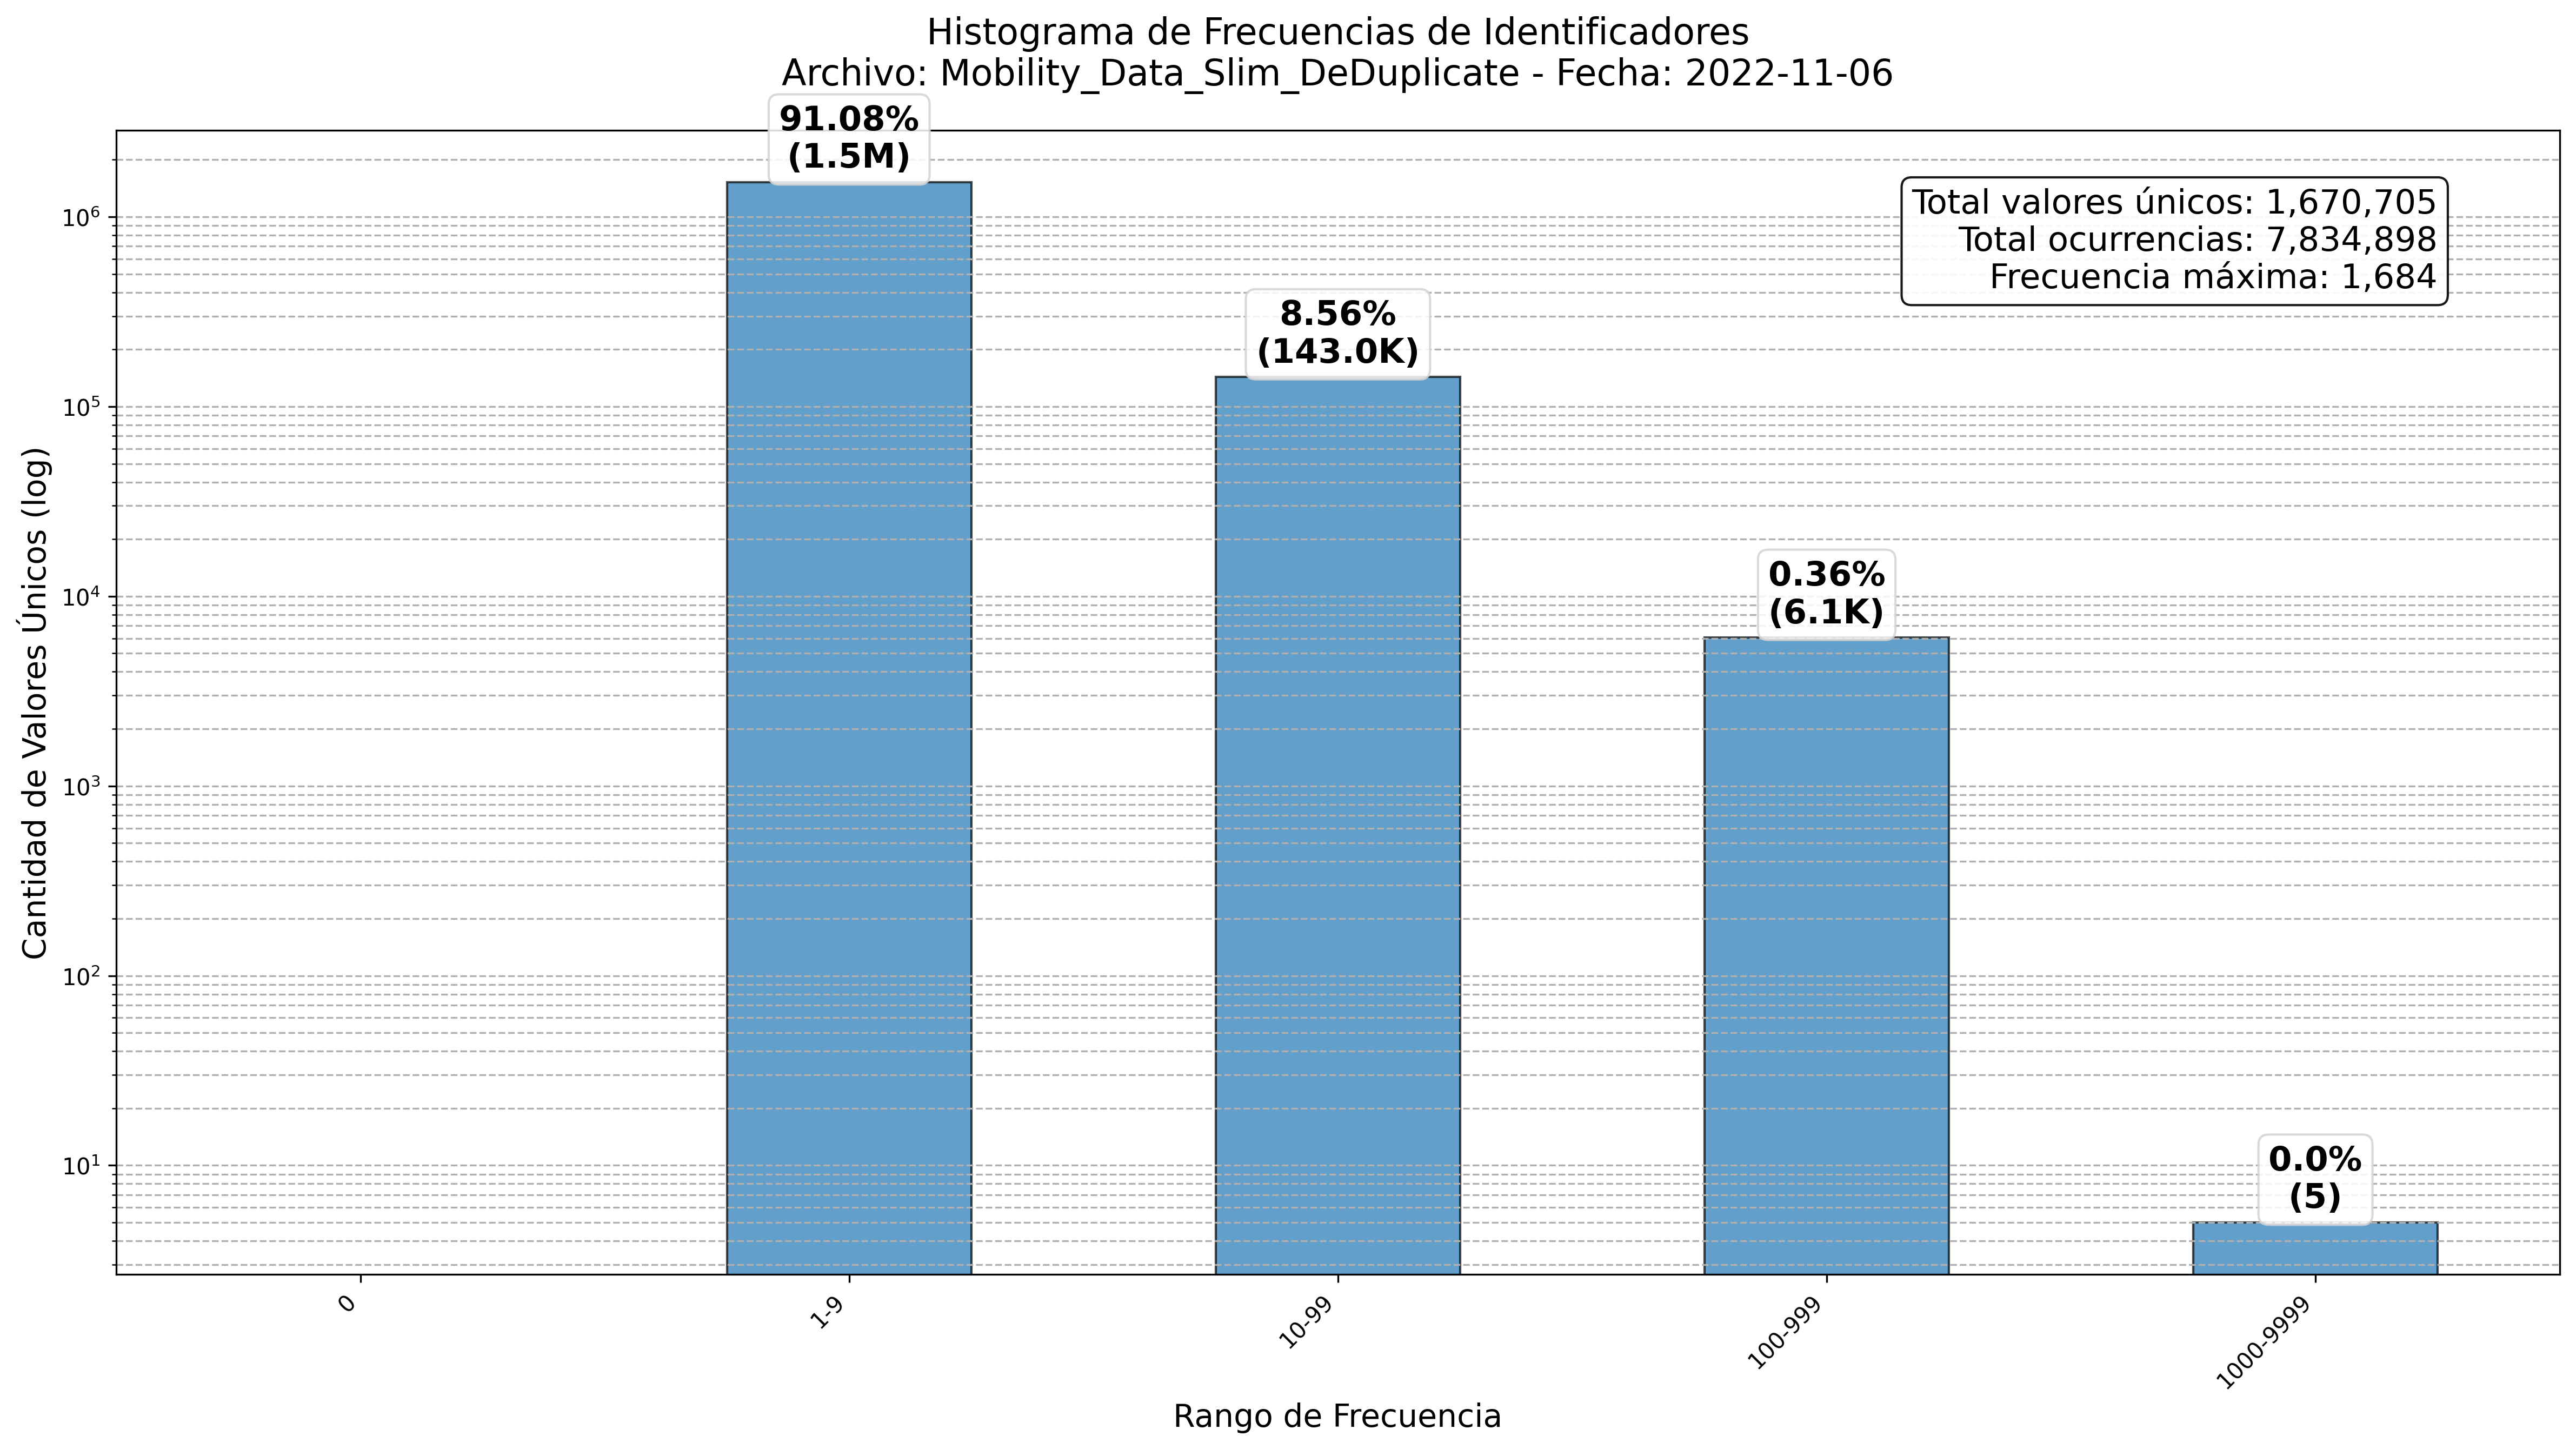
\includegraphics[width=\linewidth]{img/daily_histograms/histograma_identifier_Mobility_Data_Slim_DeDuplicate_2022-11-06.png}
        \caption{Histograma del 06/Nov/2022}
        \label{fig:sub1}
    \end{subfigure}
    \hfill
    \begin{subfigure}[t]{0.48\textwidth-1em}
        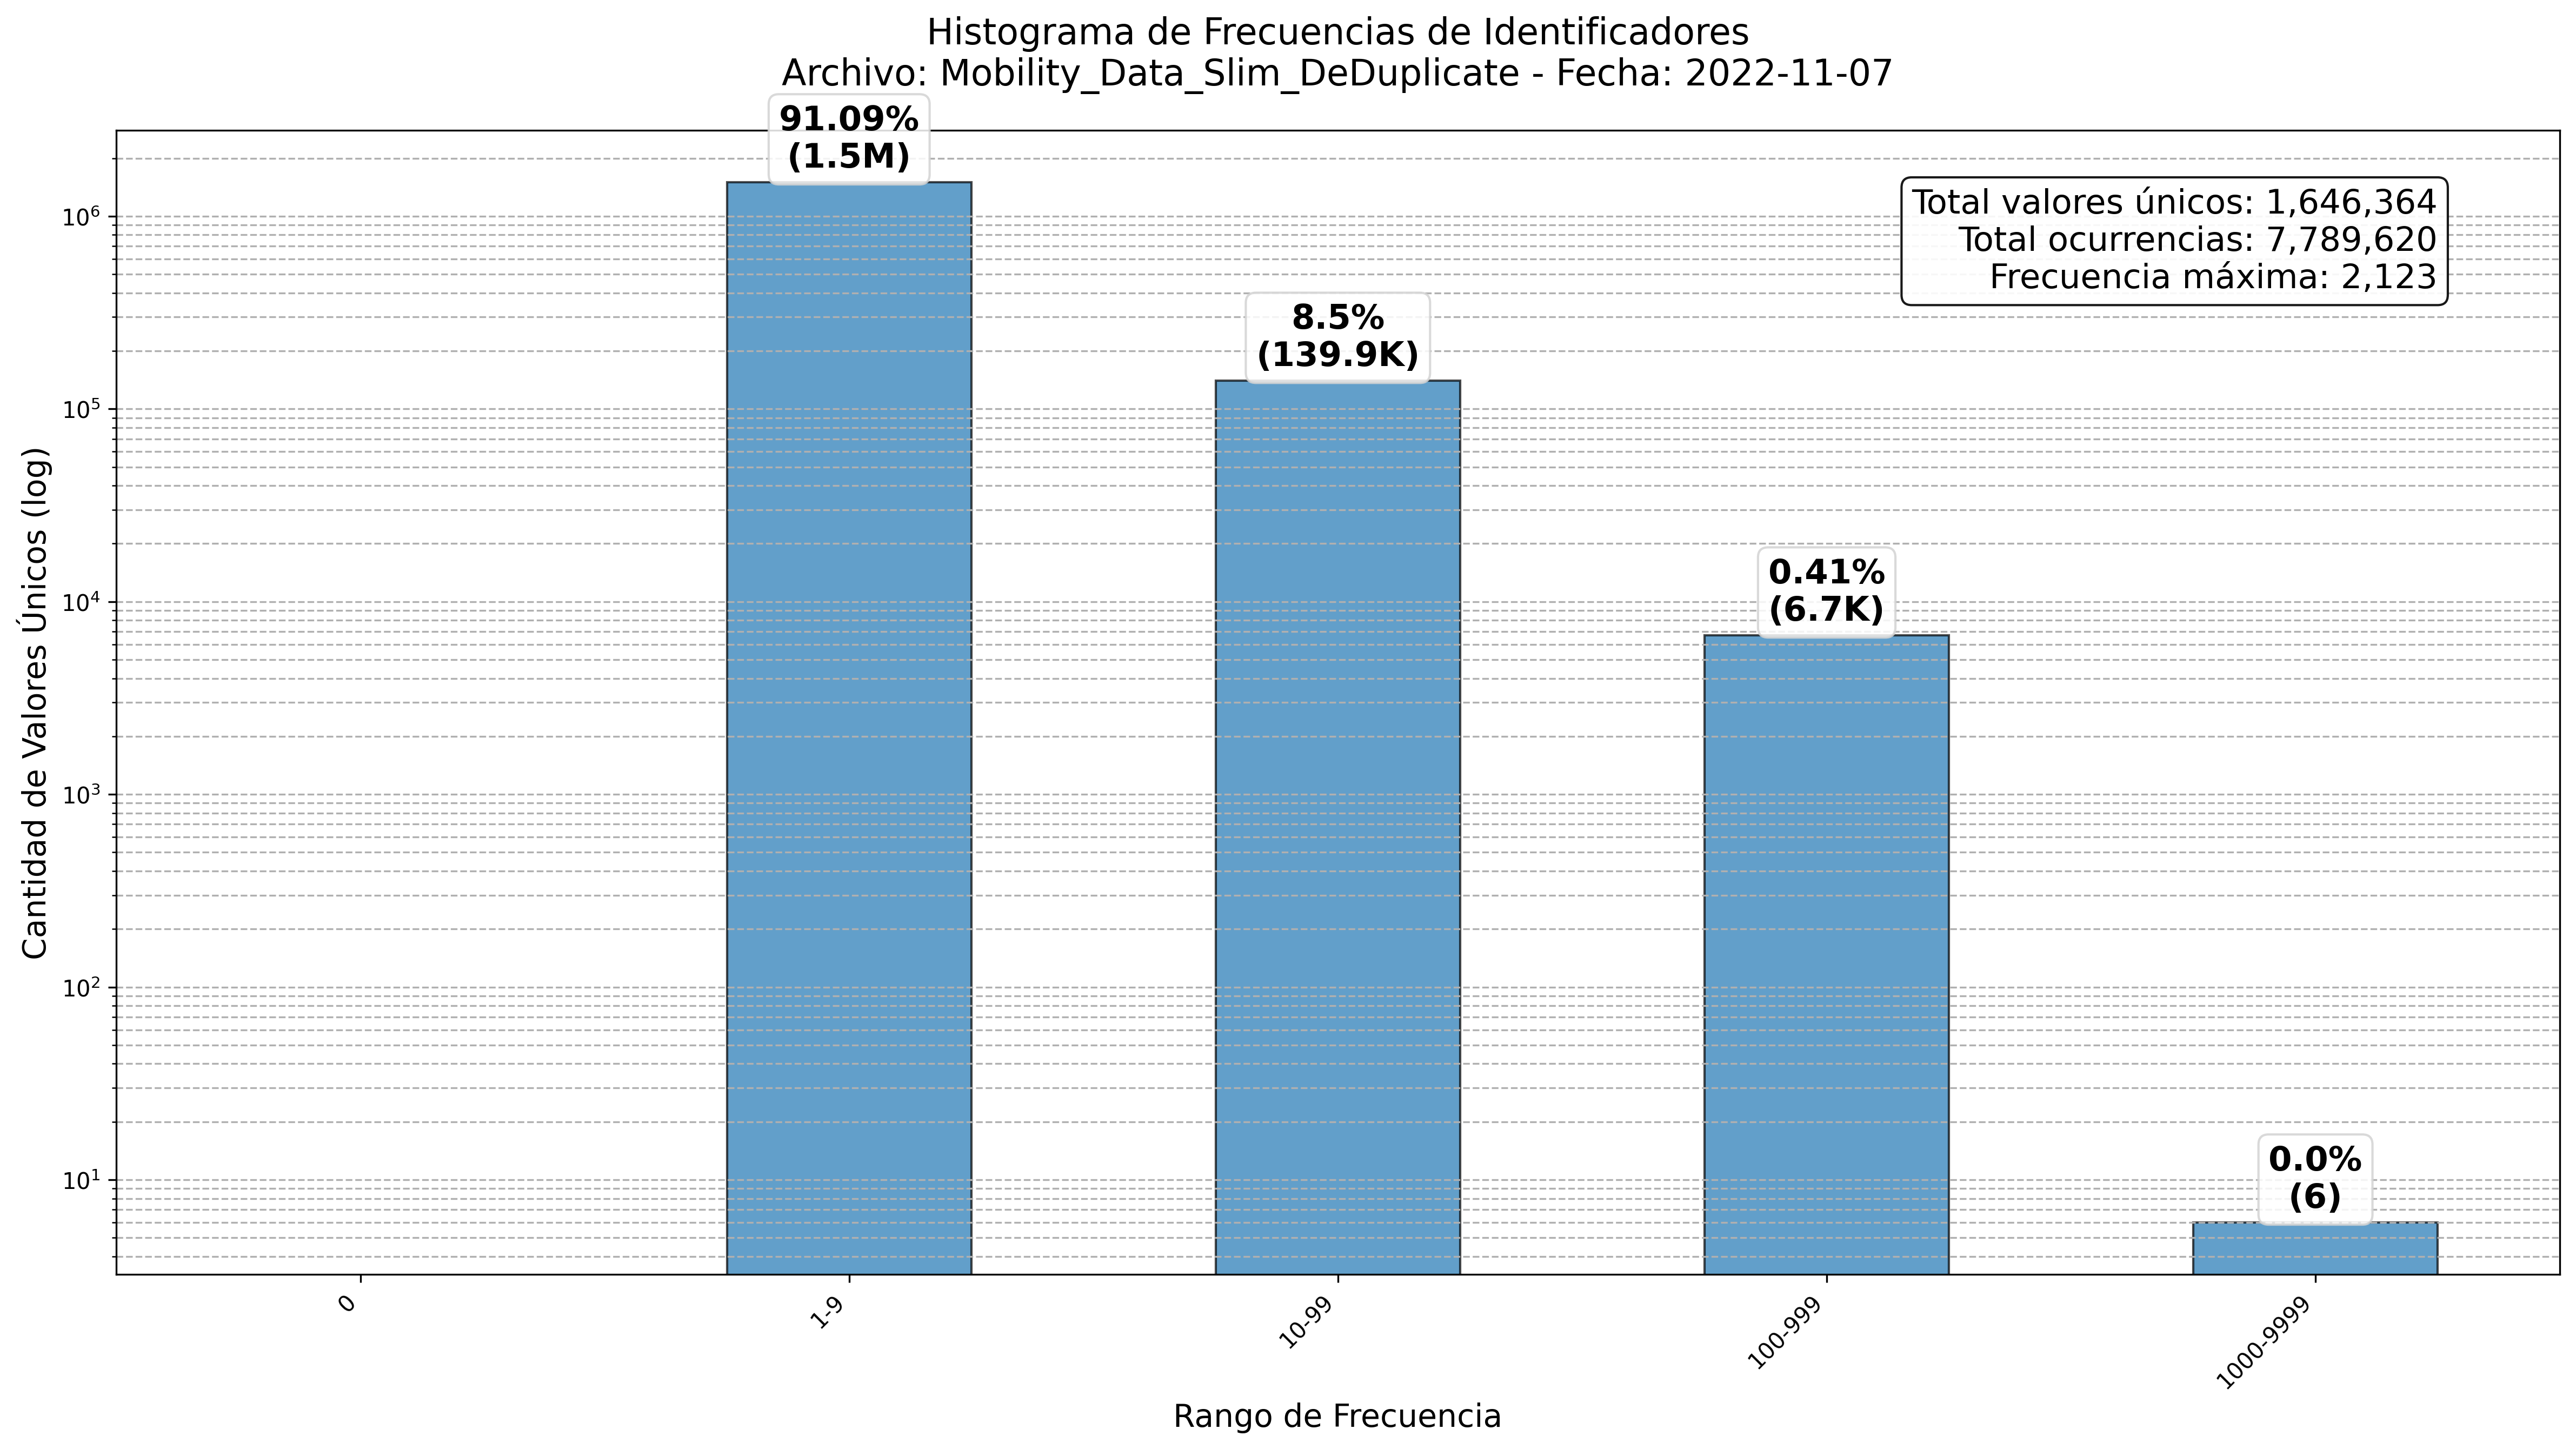
\includegraphics[width=\linewidth]{img/daily_histograms/histograma_identifier_Mobility_Data_Slim_DeDuplicate_2022-11-07.png}
        \caption{Histograma del 07/Nov/2022}
        \label{fig:sub2}
    \end{subfigure}

    \vspace{0.5cm}

    \begin{subfigure}[t]{0.48\textwidth-1em}
        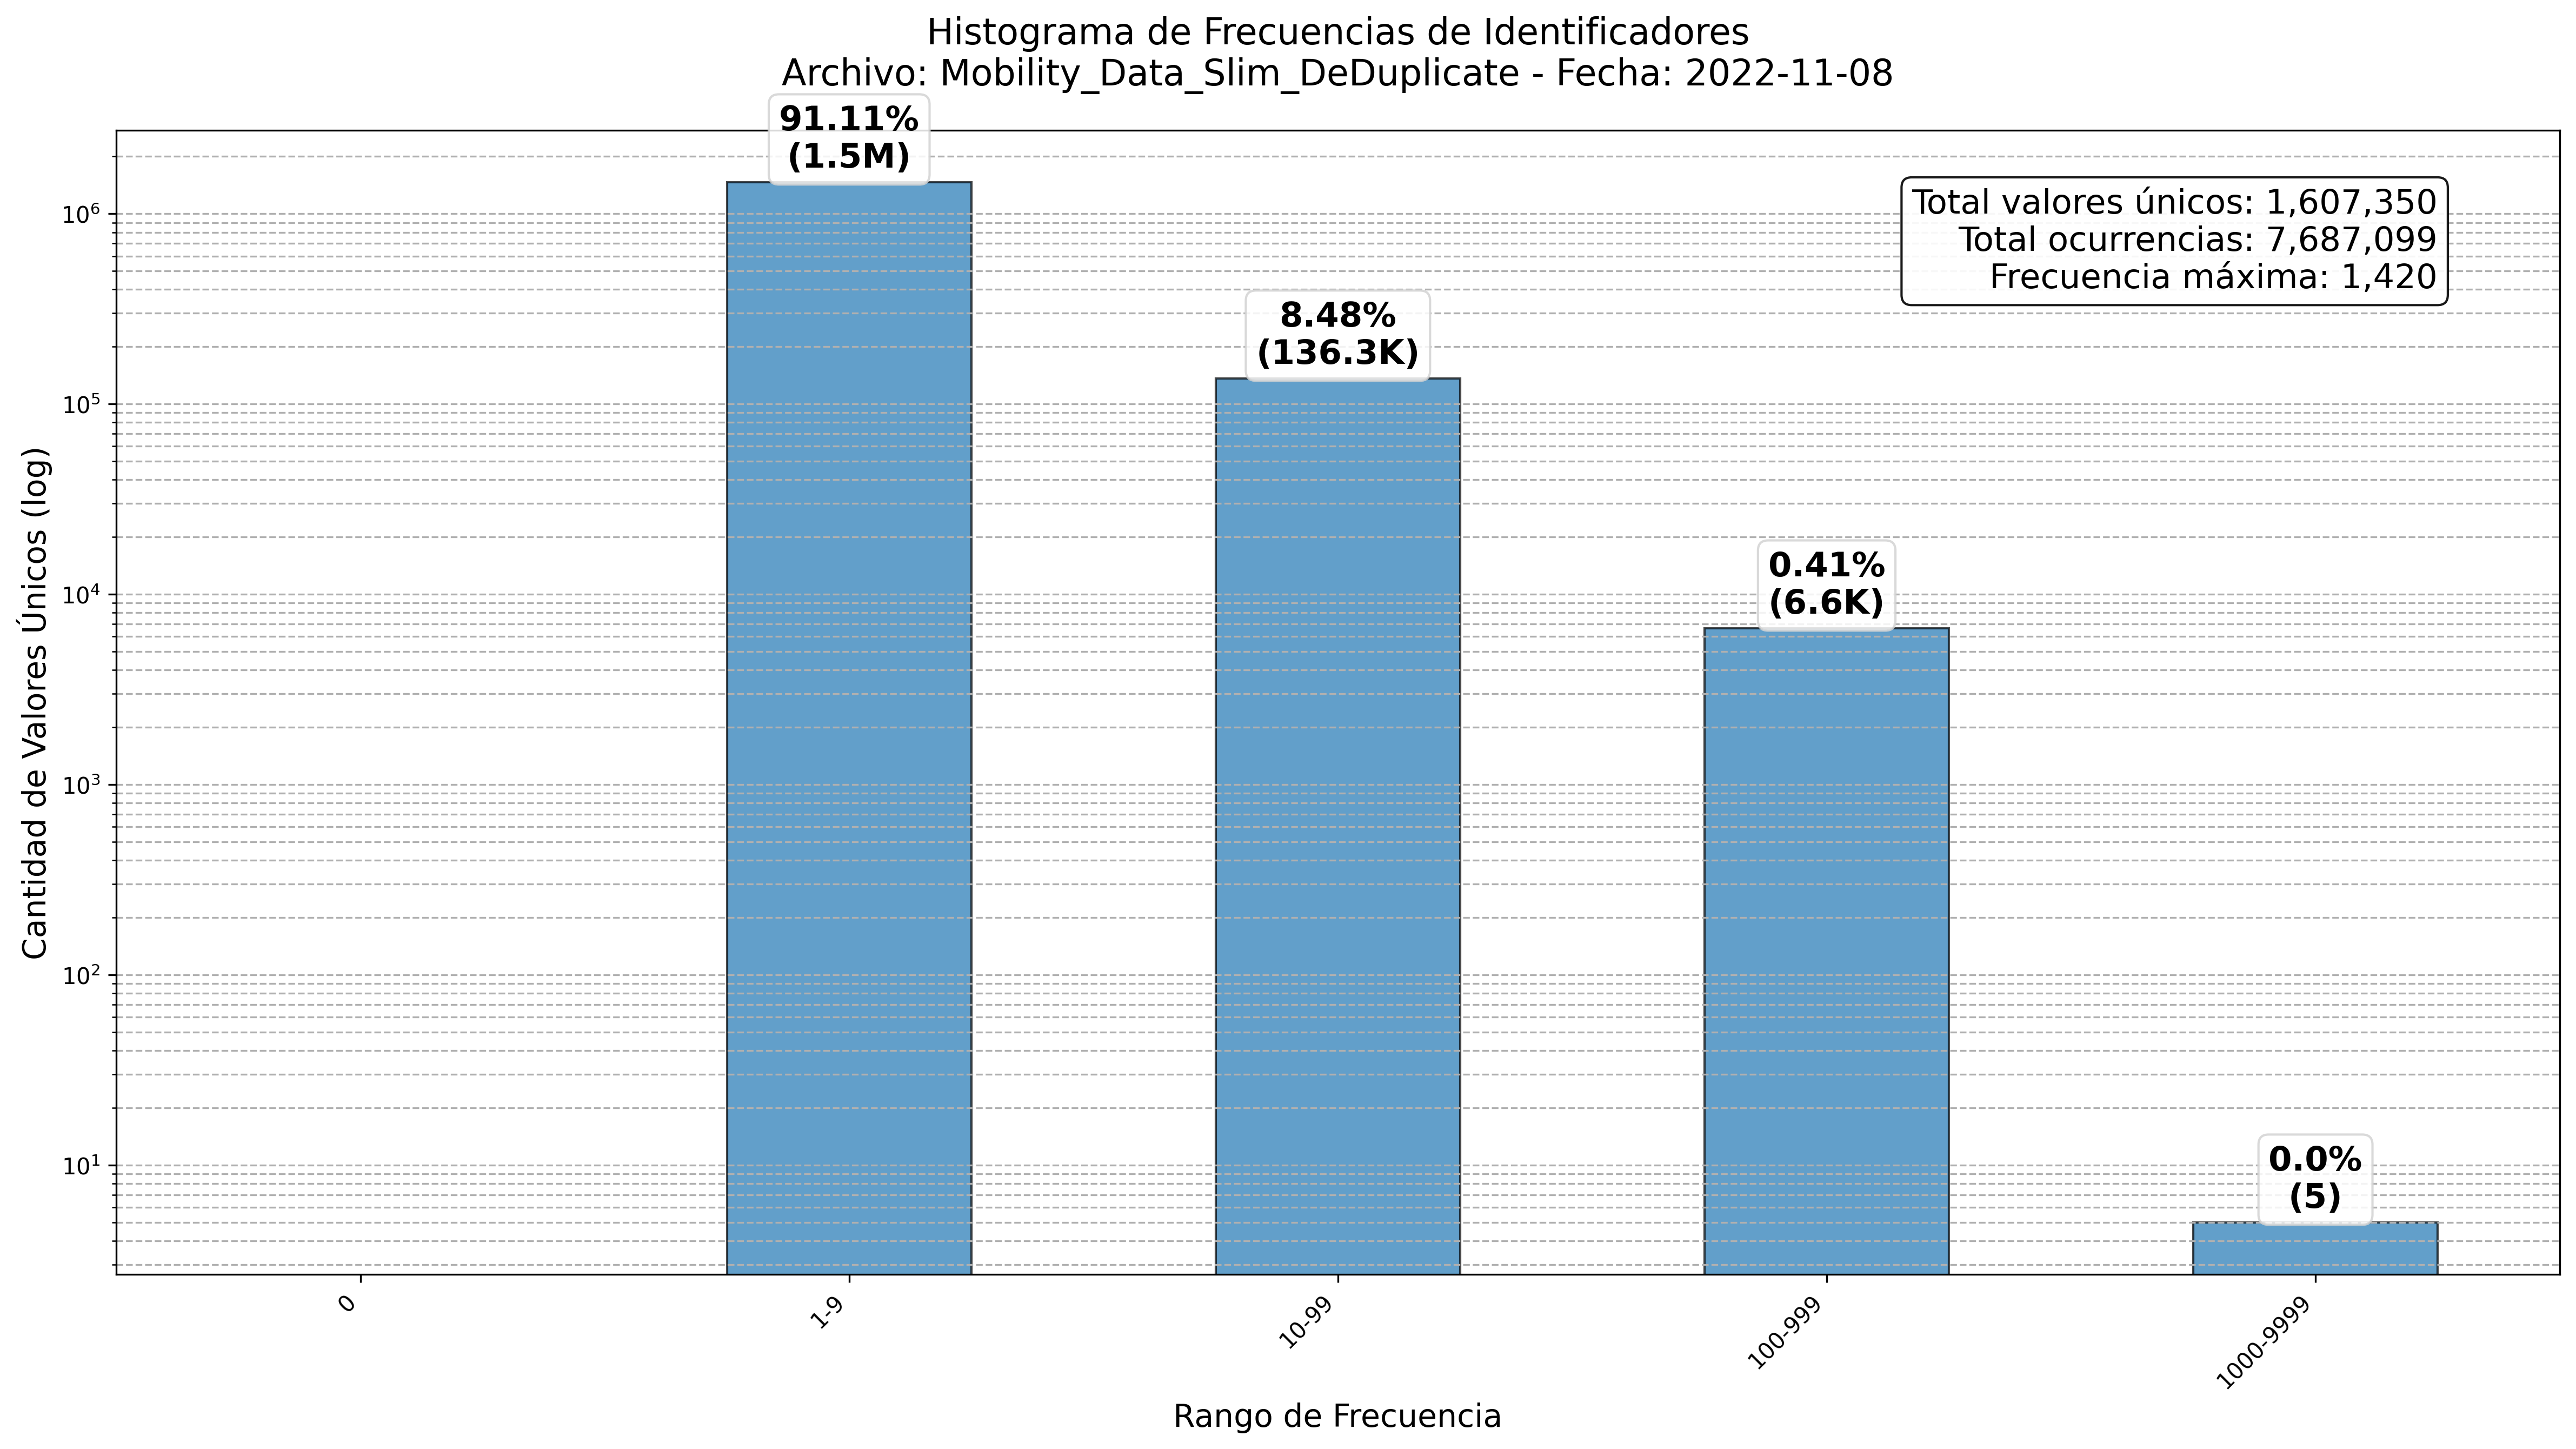
\includegraphics[width=\linewidth]{img/daily_histograms/histograma_identifier_Mobility_Data_Slim_DeDuplicate_2022-11-08.png}
        \caption{Histograma del 08/Nov/2022}
        \label{fig:sub3}
    \end{subfigure}
    \hfill
    \begin{subfigure}[t]{0.48\textwidth-1em}
        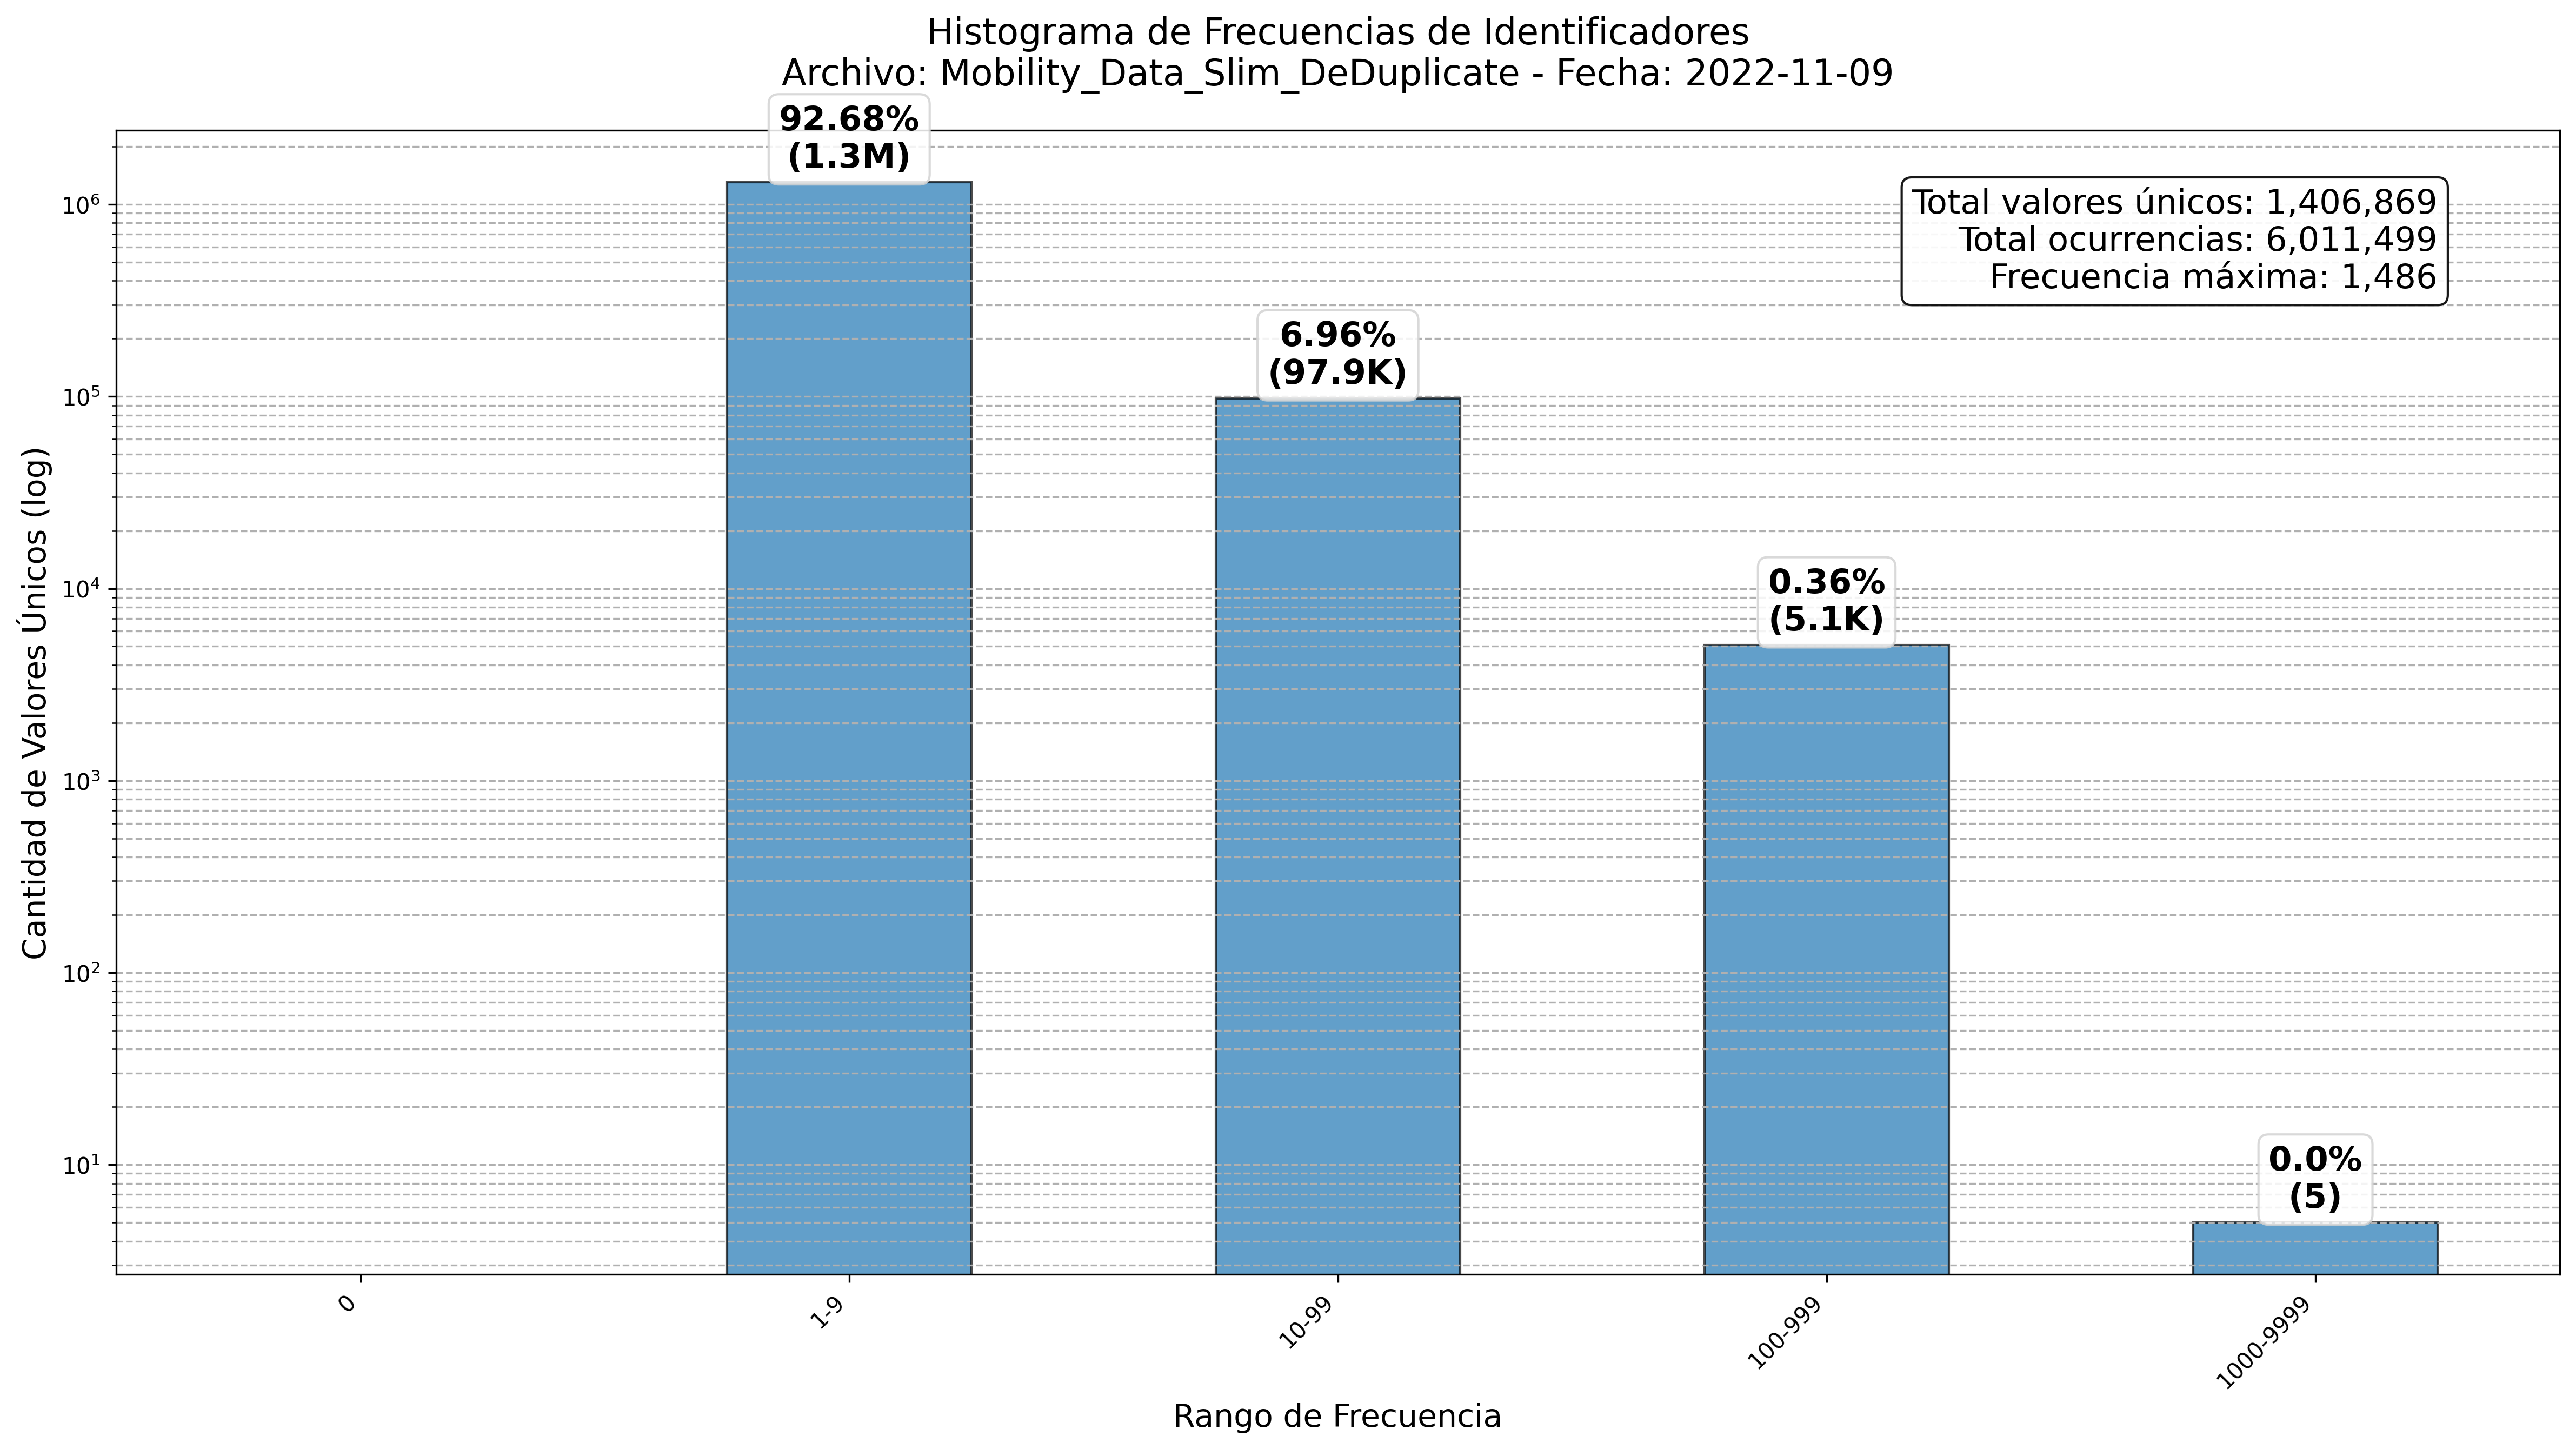
\includegraphics[width=\linewidth]{img/daily_histograms/histograma_identifier_Mobility_Data_Slim_DeDuplicate_2022-11-09.png}
        \caption{Histograma del 09/Nov/2022}
        \label{fig:sub4}
    \end{subfigure}
\end{figure}

\begin{figure}[H]
    \ContinuedFloat
    \centering
    \begin{subfigure}[t]{0.48\textwidth-1em}
        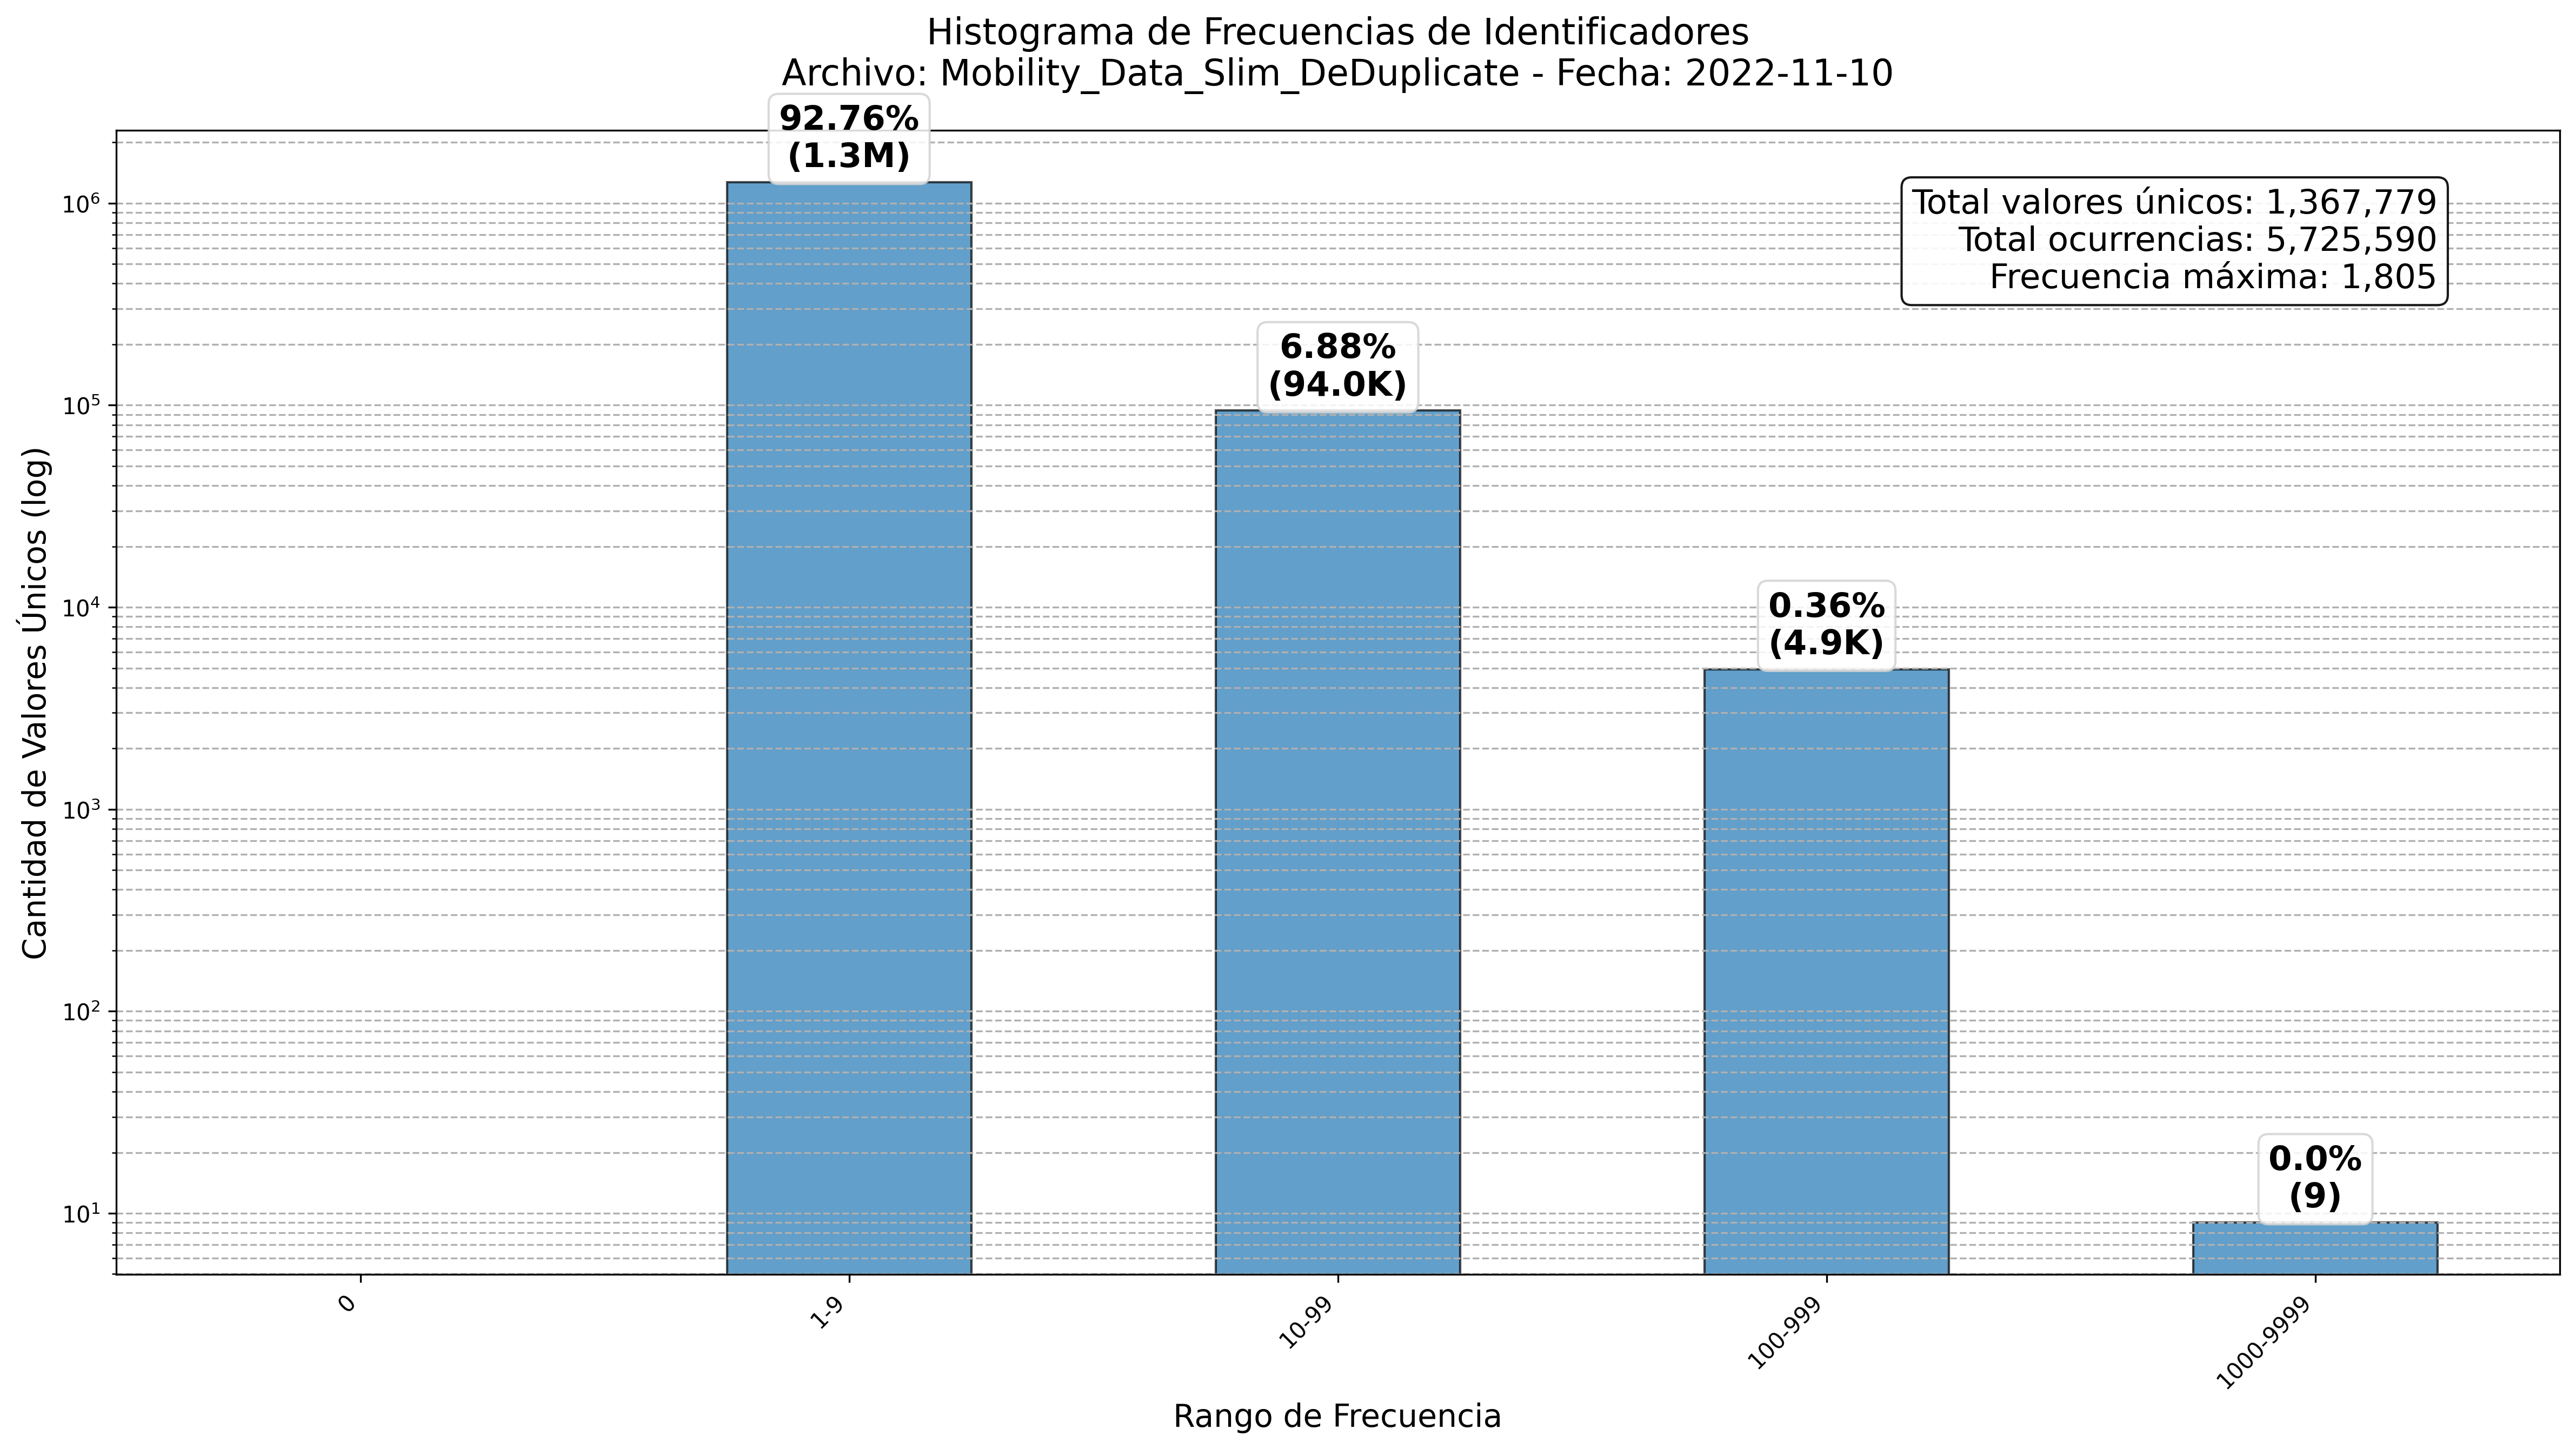
\includegraphics[width=\linewidth]{img/daily_histograms/histograma_identifier_Mobility_Data_Slim_DeDuplicate_2022-11-10.png}
        \caption{Histograma del 10/Nov/2022}
        \label{fig:sub5}
    \end{subfigure}
    \hfill
    \begin{subfigure}[t]{0.48\textwidth-1em}
        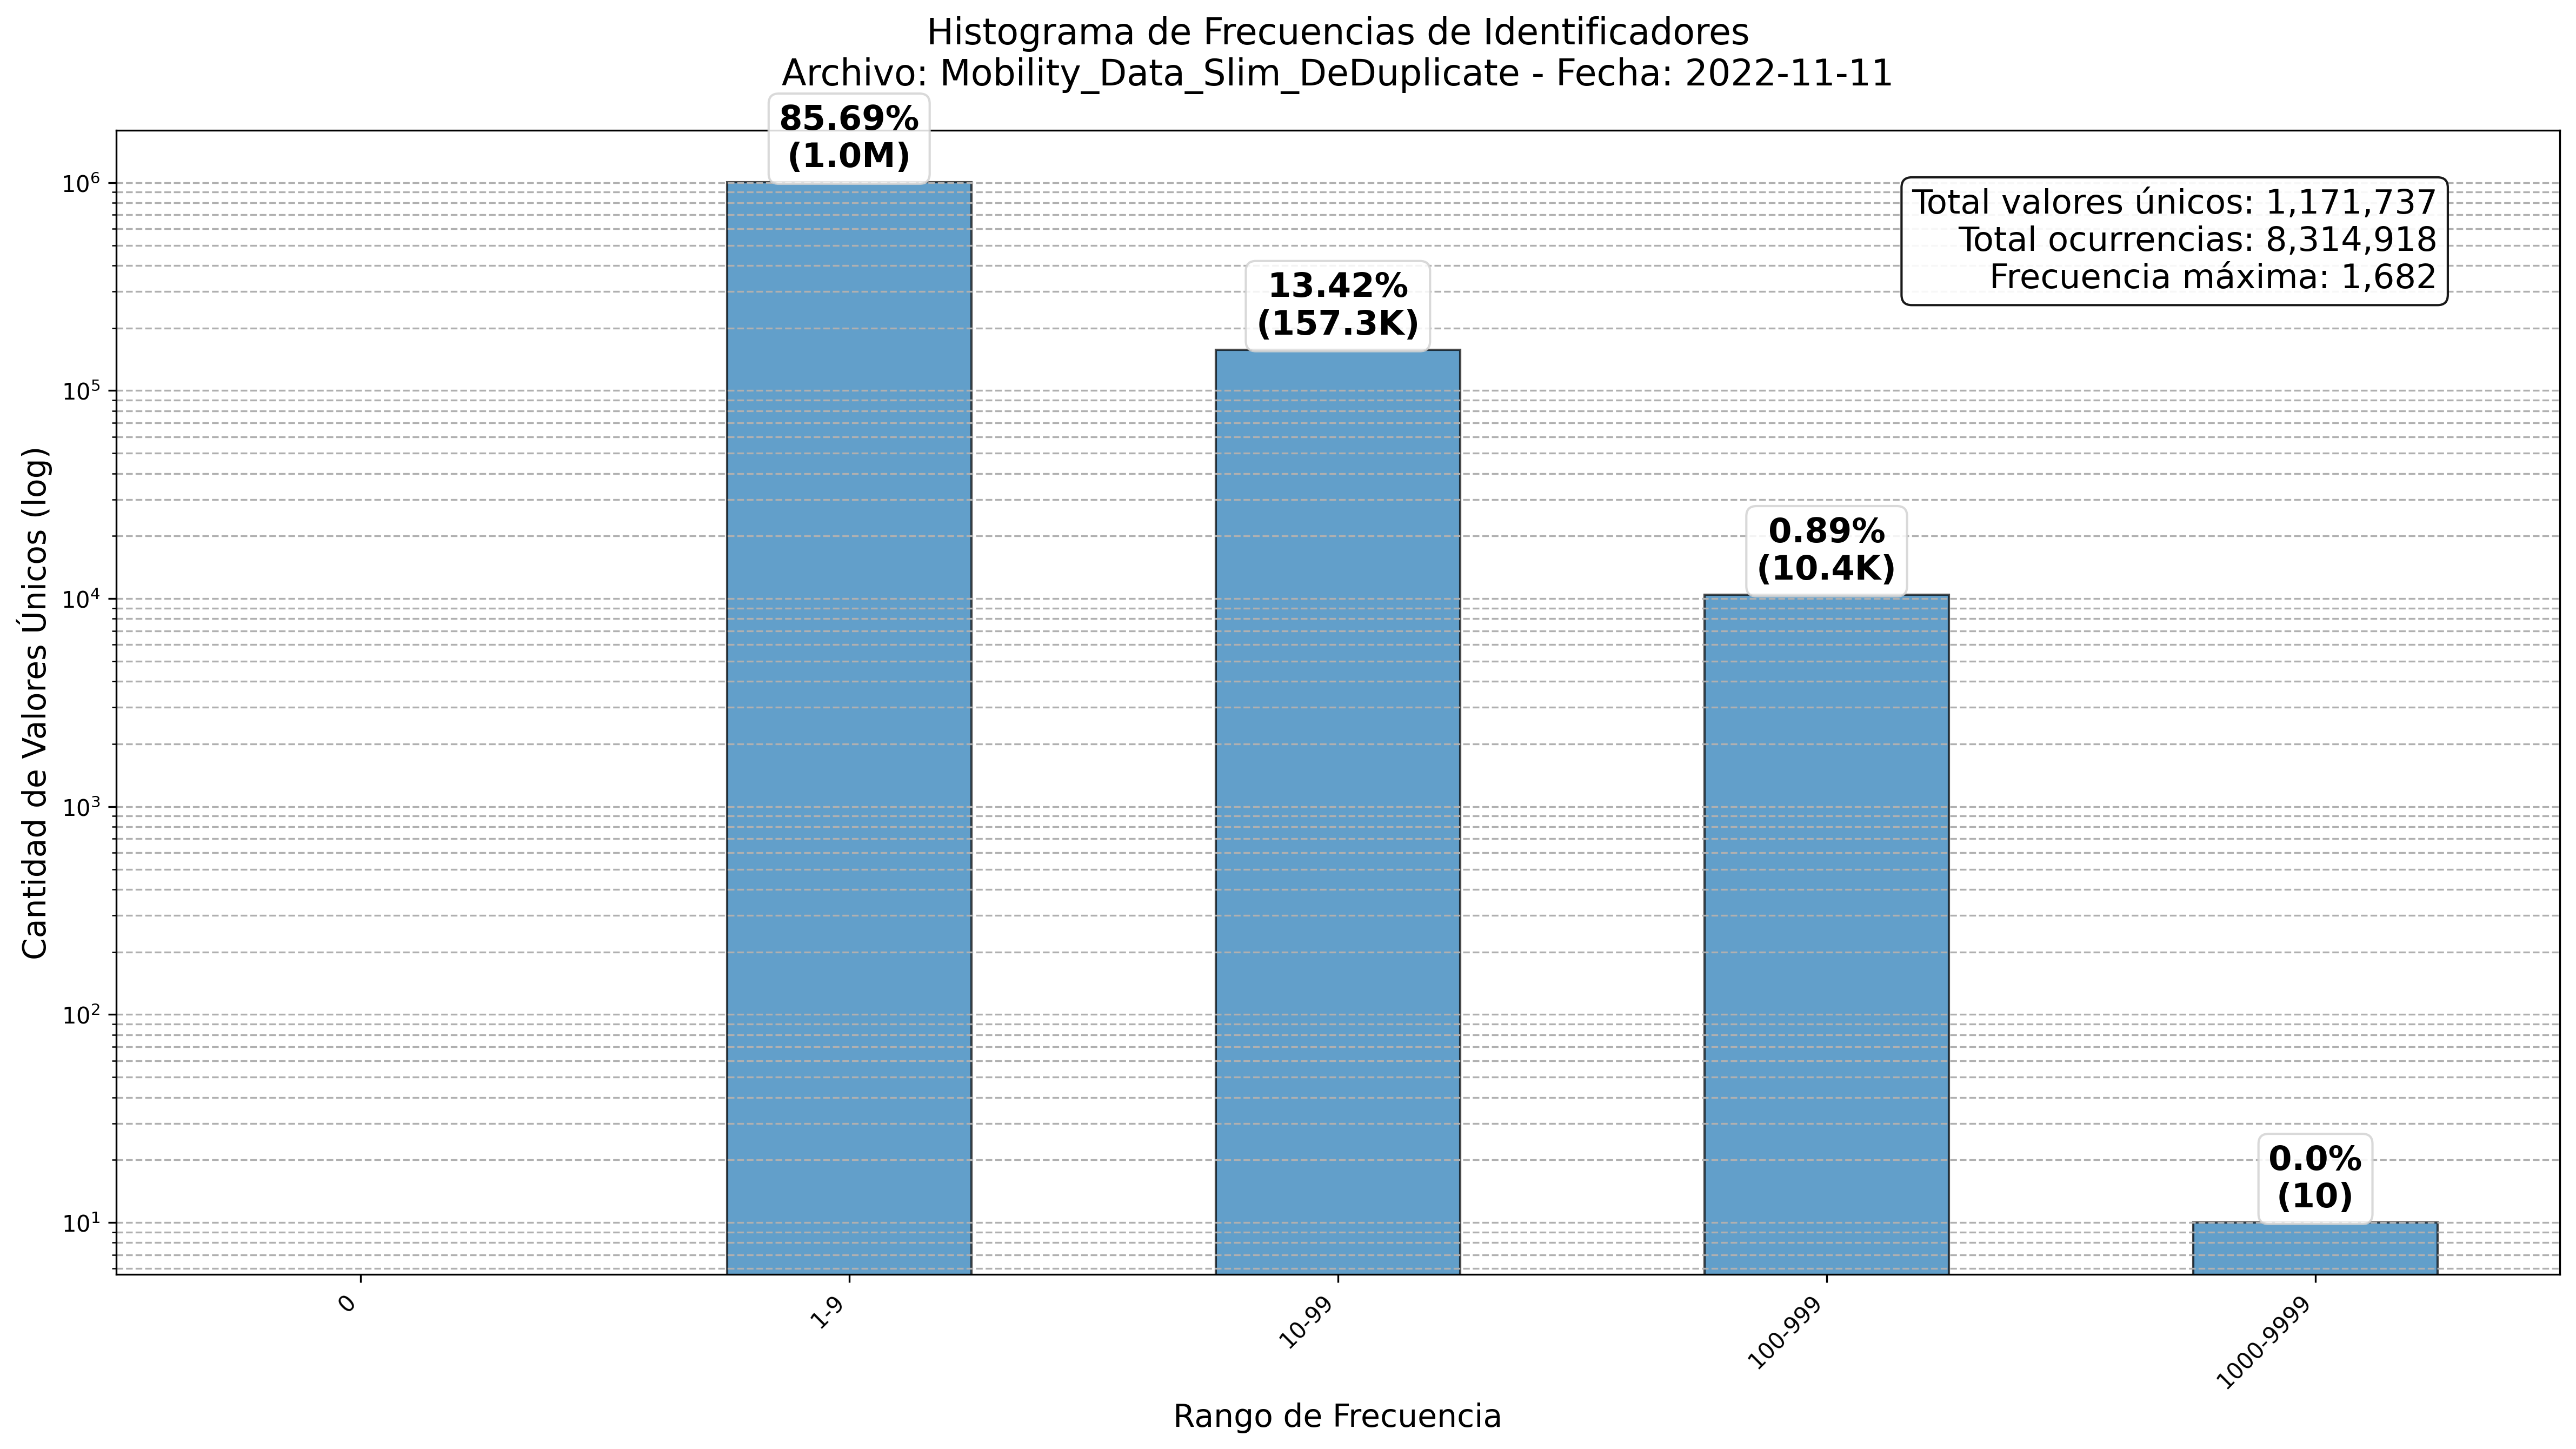
\includegraphics[width=\linewidth]{img/daily_histograms/histograma_identifier_Mobility_Data_Slim_DeDuplicate_2022-11-11.png}
        \caption{Histograma del 11/Nov/2022}
        \label{fig:sub6}
    \end{subfigure}

    \vspace{0.5cm}

    \begin{subfigure}[t]{0.48\textwidth-1em}
        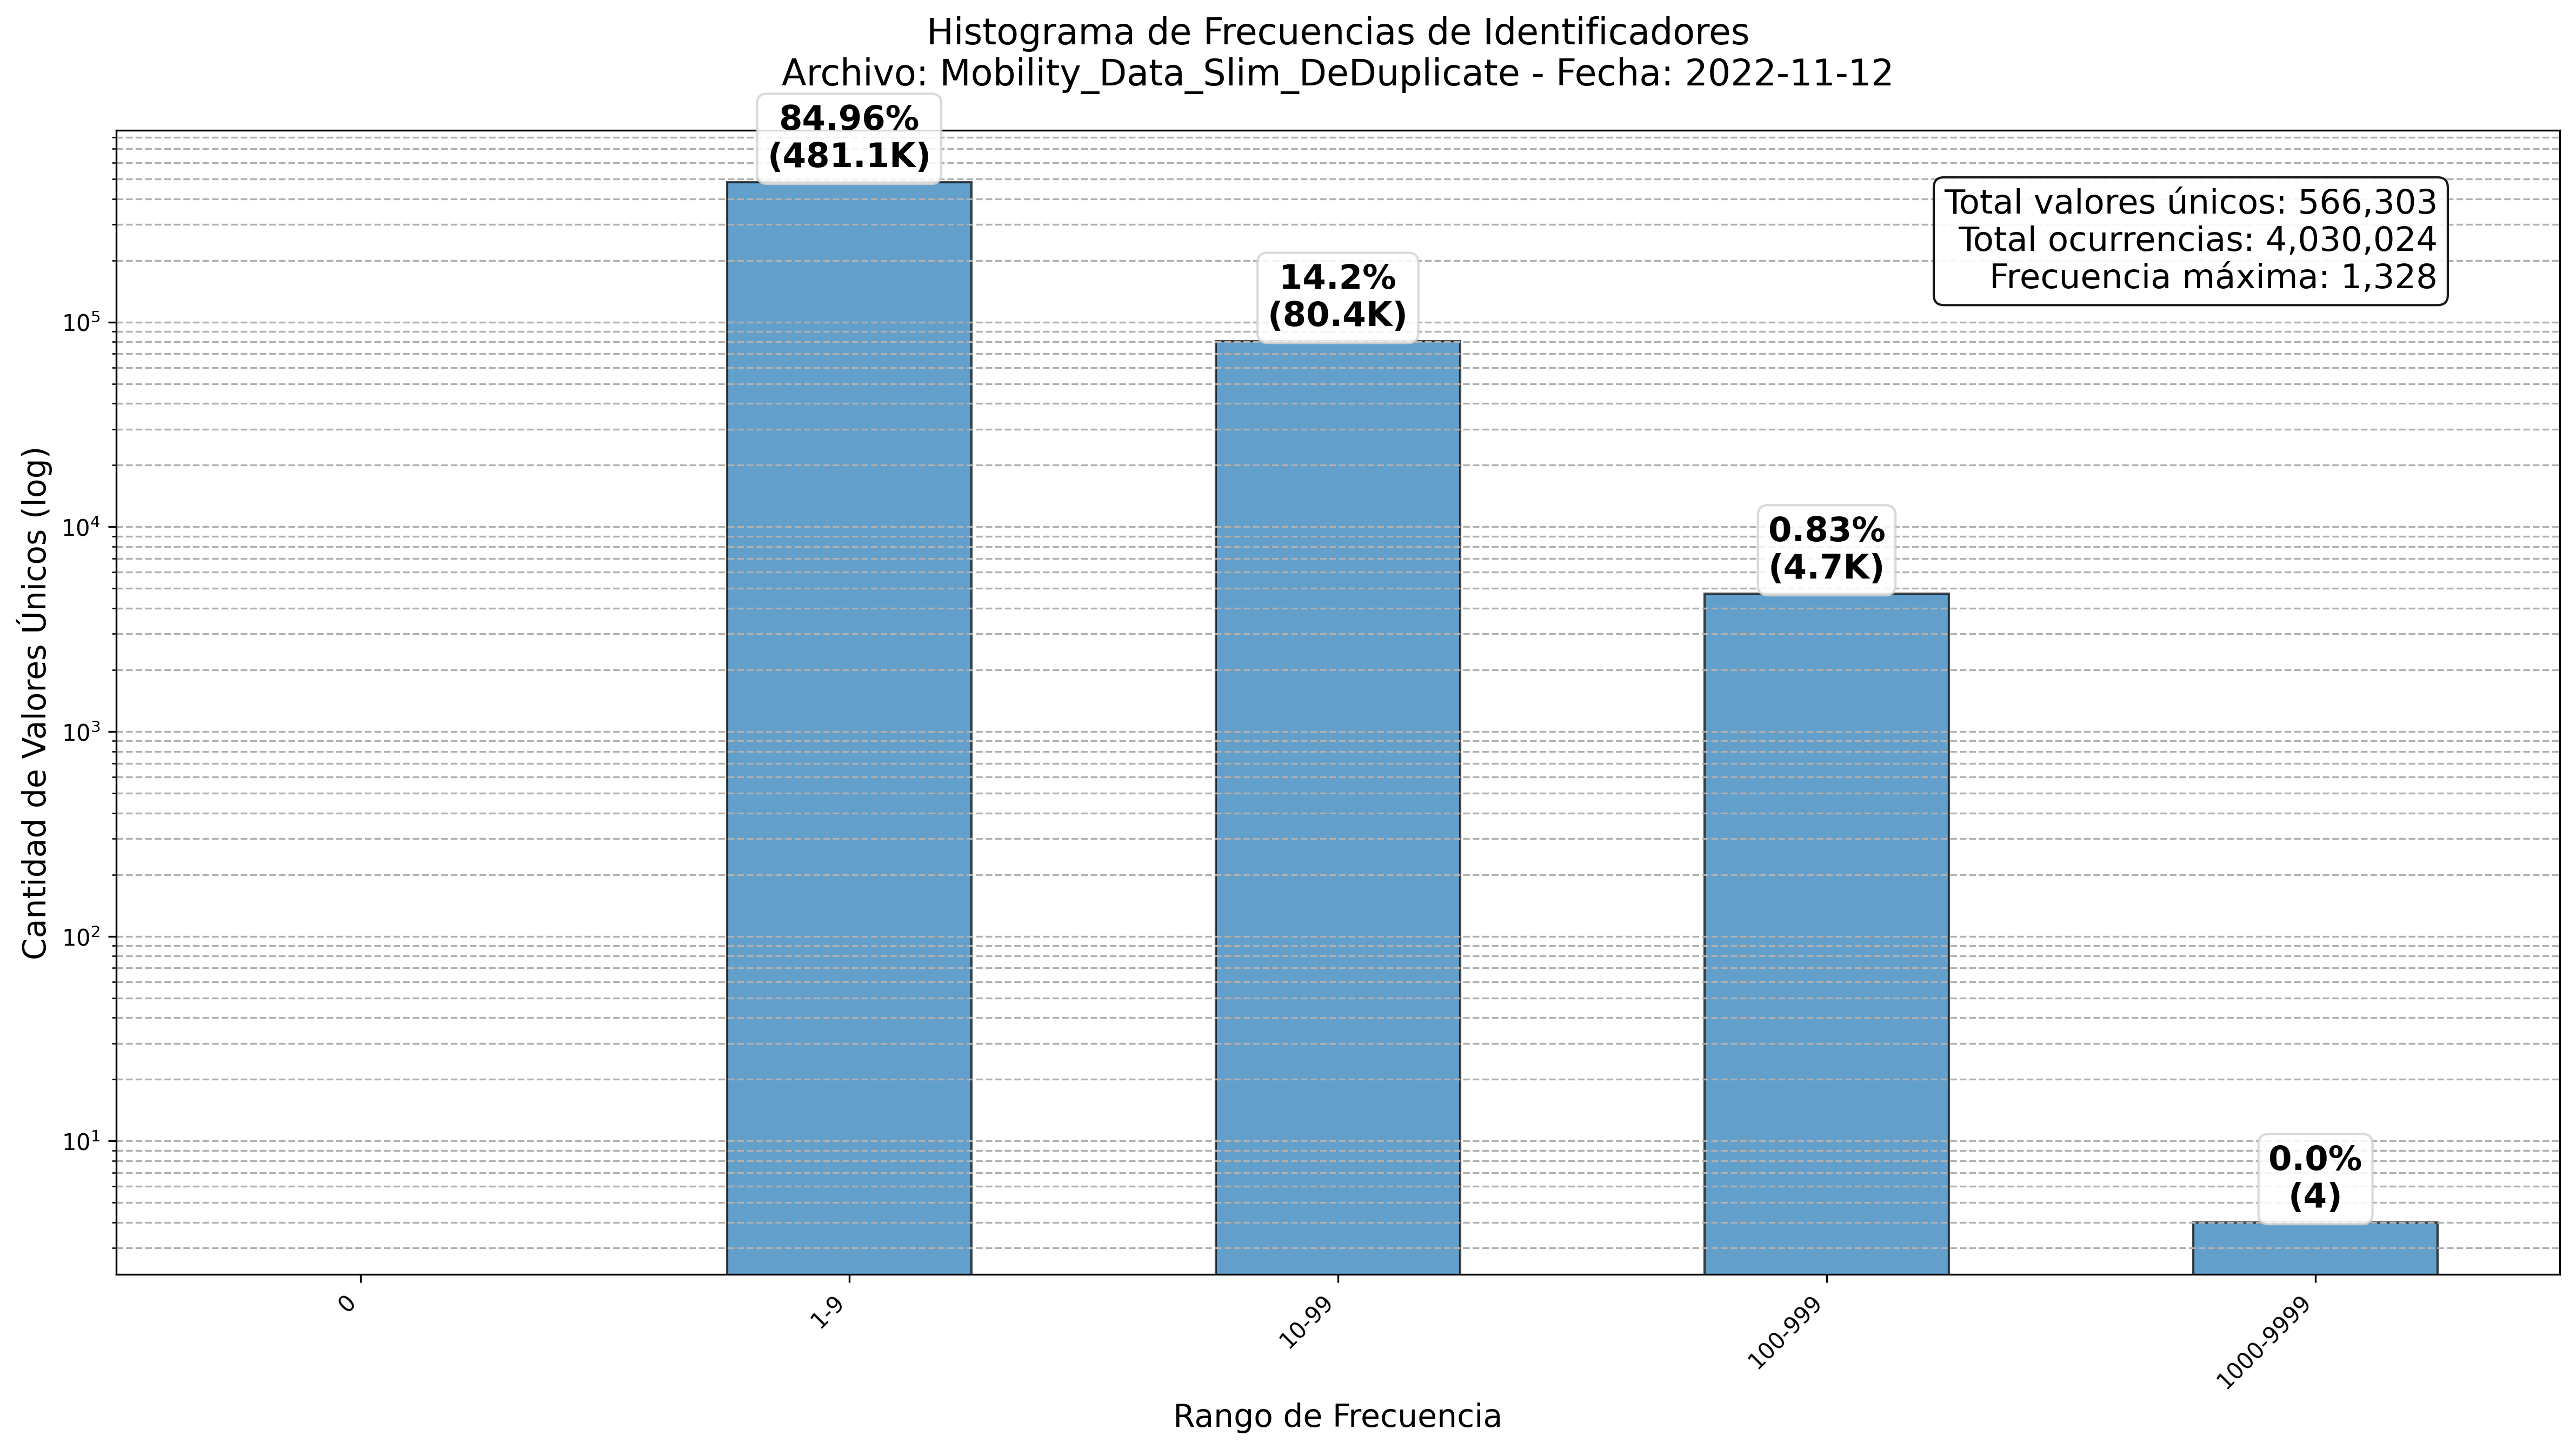
\includegraphics[width=\linewidth]{img/daily_histograms/histograma_identifier_Mobility_Data_Slim_DeDuplicate_2022-11-12.png}
        \caption{Histograma del 12/Nov/2022}
        \label{fig:sub7}
    \end{subfigure}
    \hfill
    \begin{subfigure}[t]{0.48\textwidth-1em}
        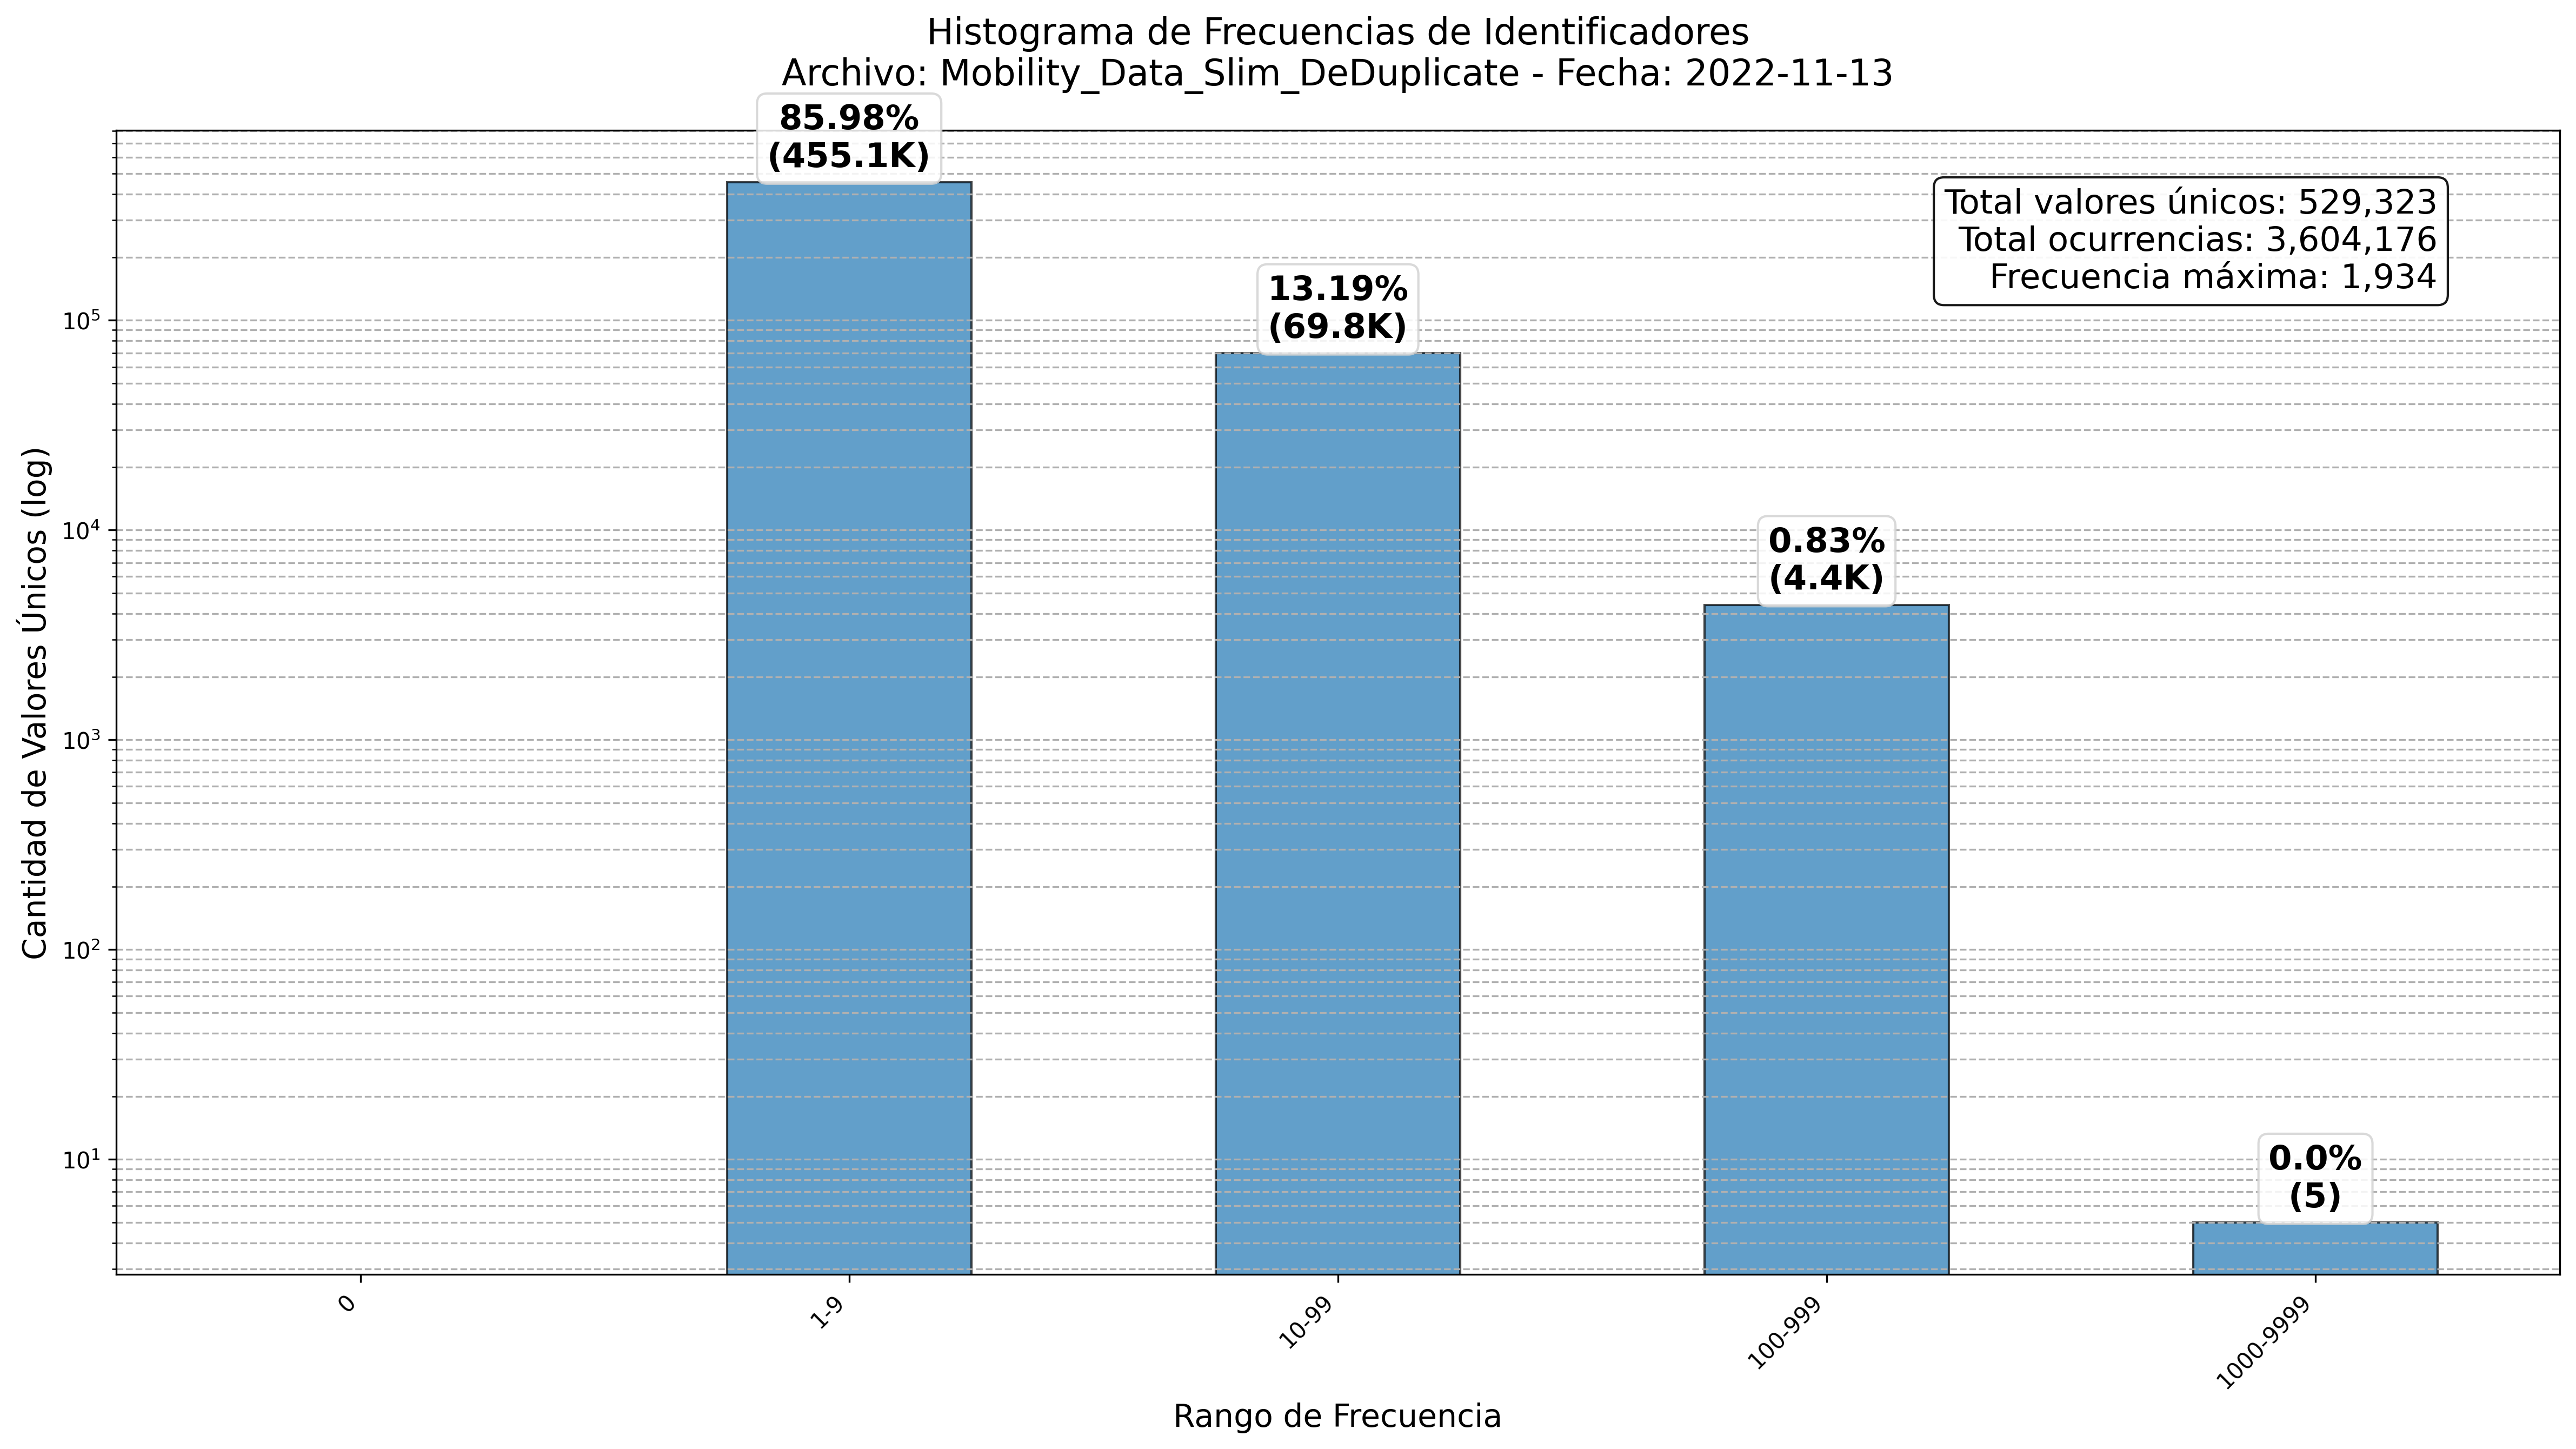
\includegraphics[width=\linewidth]{img/daily_histograms/histograma_identifier_Mobility_Data_Slim_DeDuplicate_2022-11-13.png}
        \caption{Histograma del 13/Nov/2022}
        \label{fig:sub8}
    \end{subfigure}

    \vspace{0.5cm}

    \begin{subfigure}[t]{0.48\textwidth-1em}
        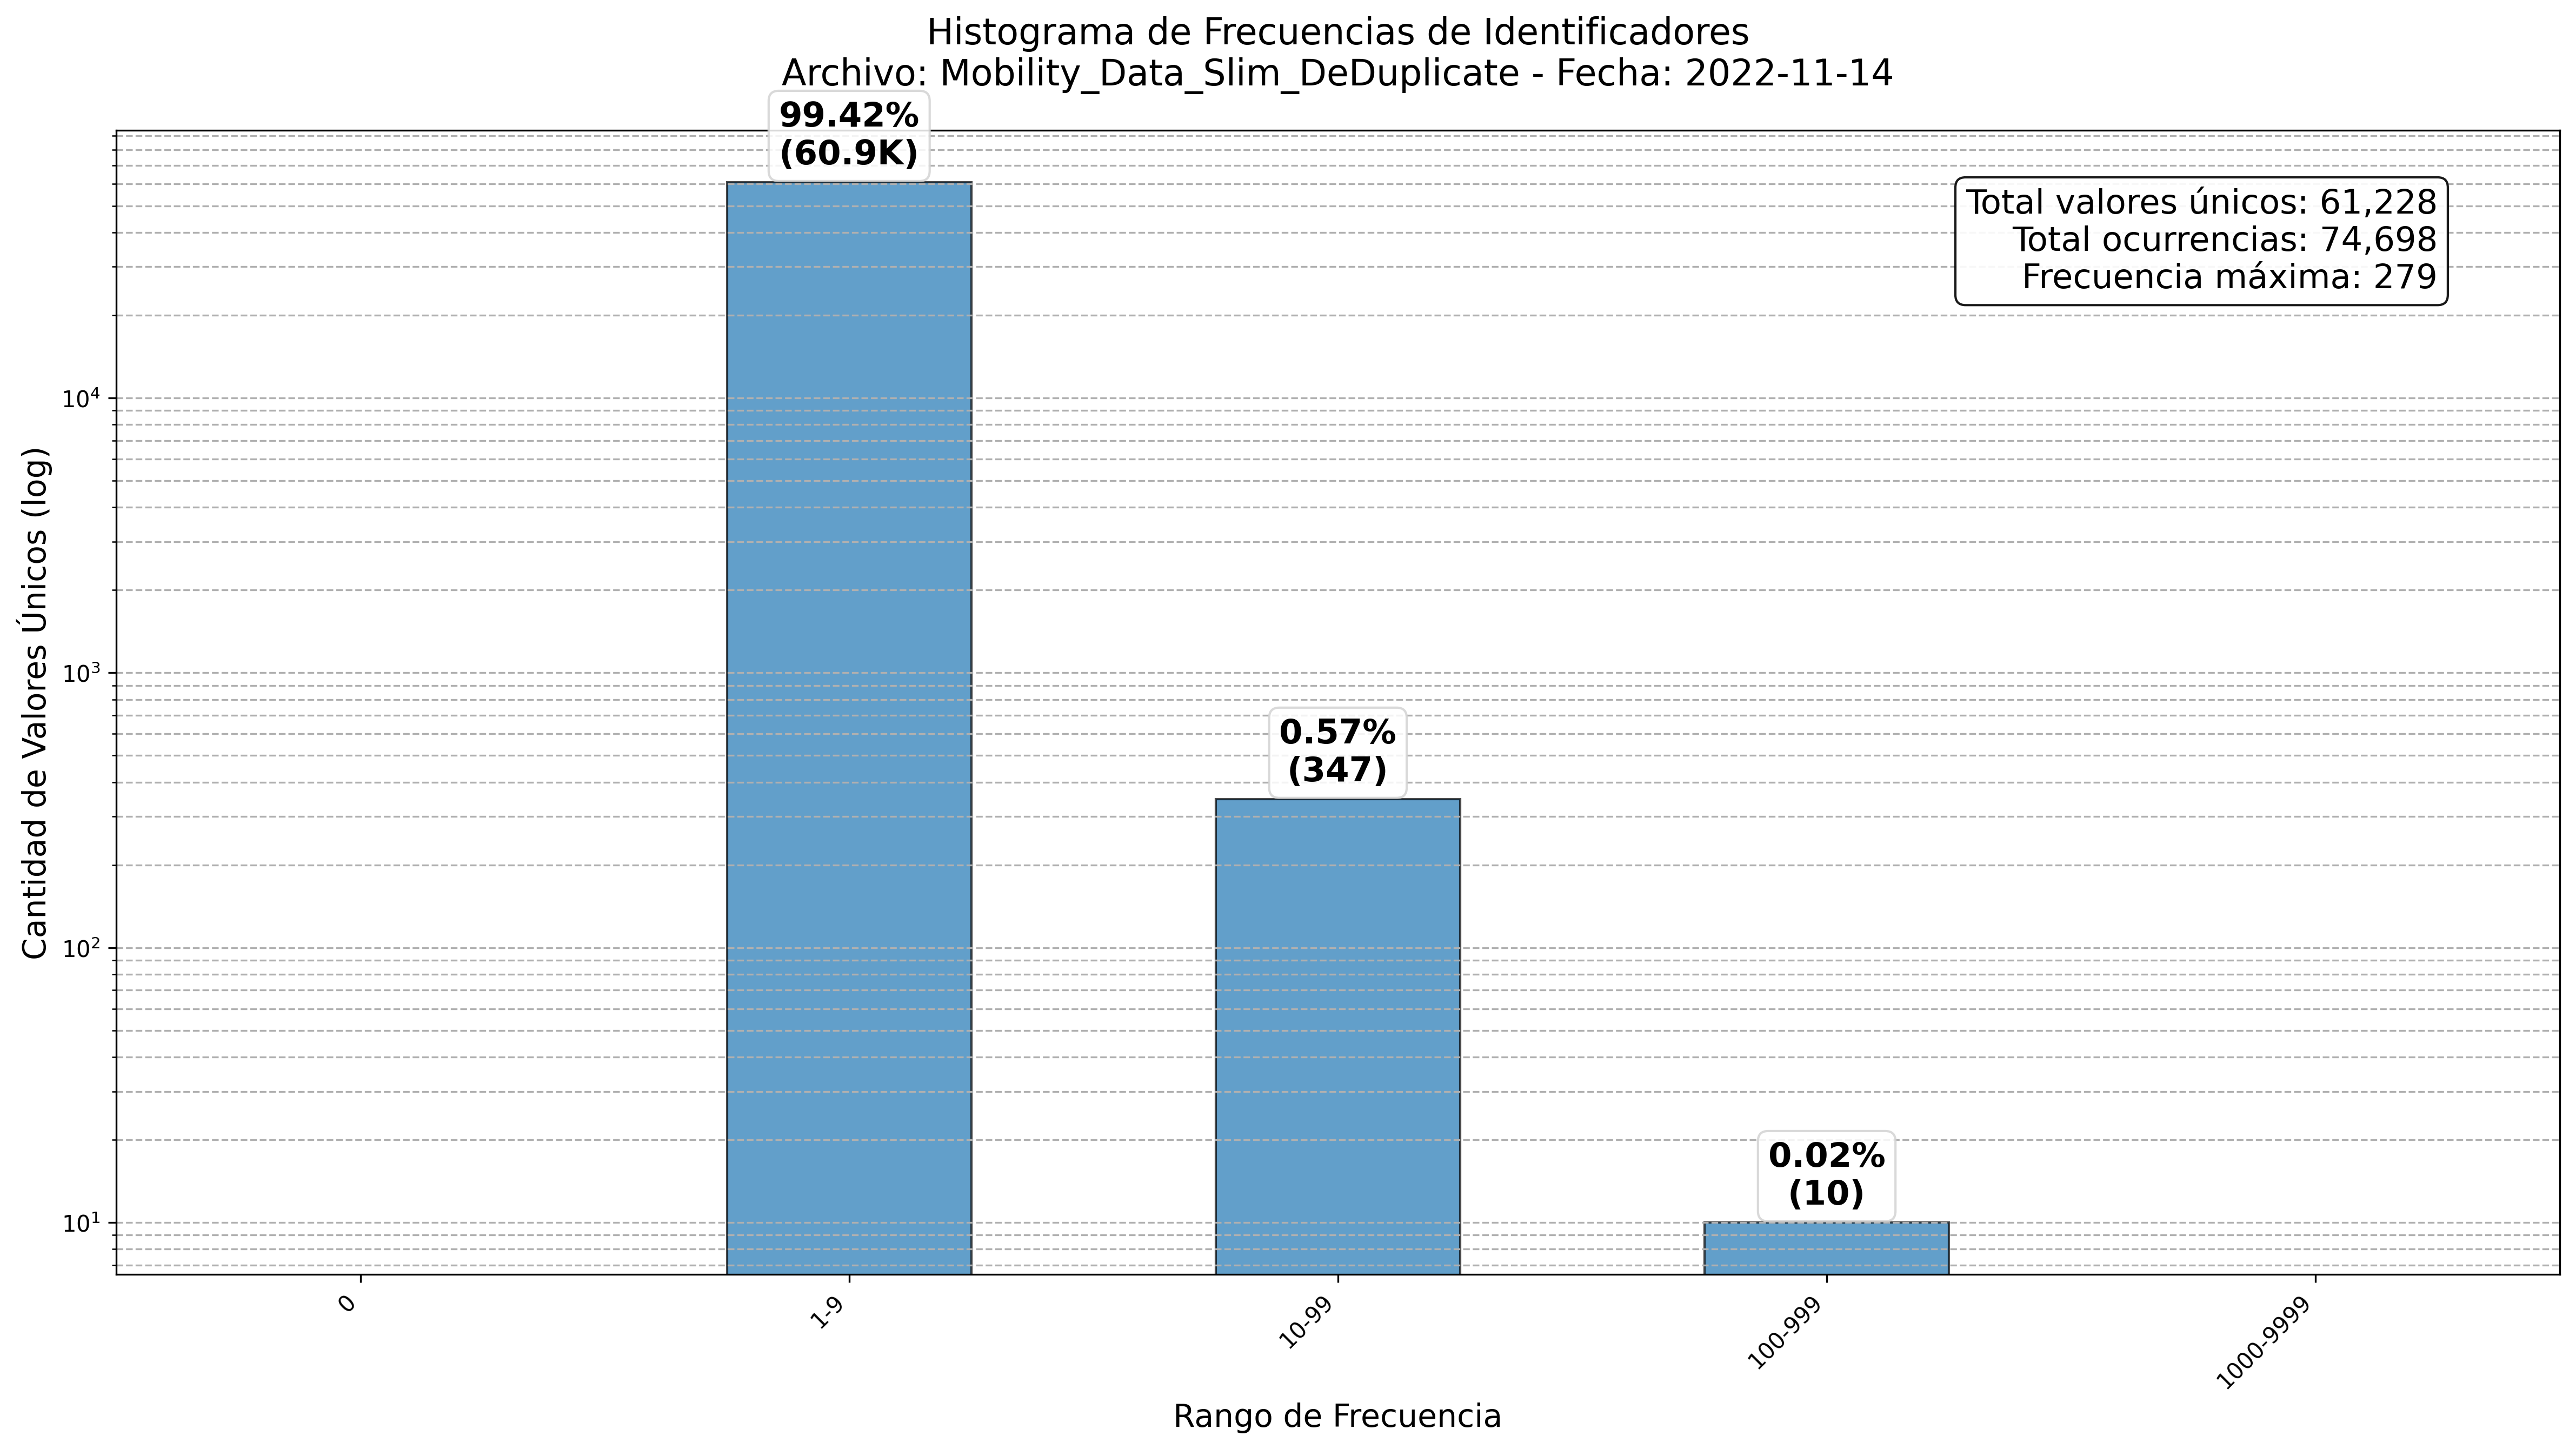
\includegraphics[width=\linewidth]{img/daily_histograms/histograma_identifier_Mobility_Data_Slim_DeDuplicate_2022-11-14.png}
        \caption{Histograma del 14/Nov/2022}
        \label{fig:sub9}
    \end{subfigure}
    \hfill
    \begin{subfigure}[t]{0.48\textwidth-1em}
        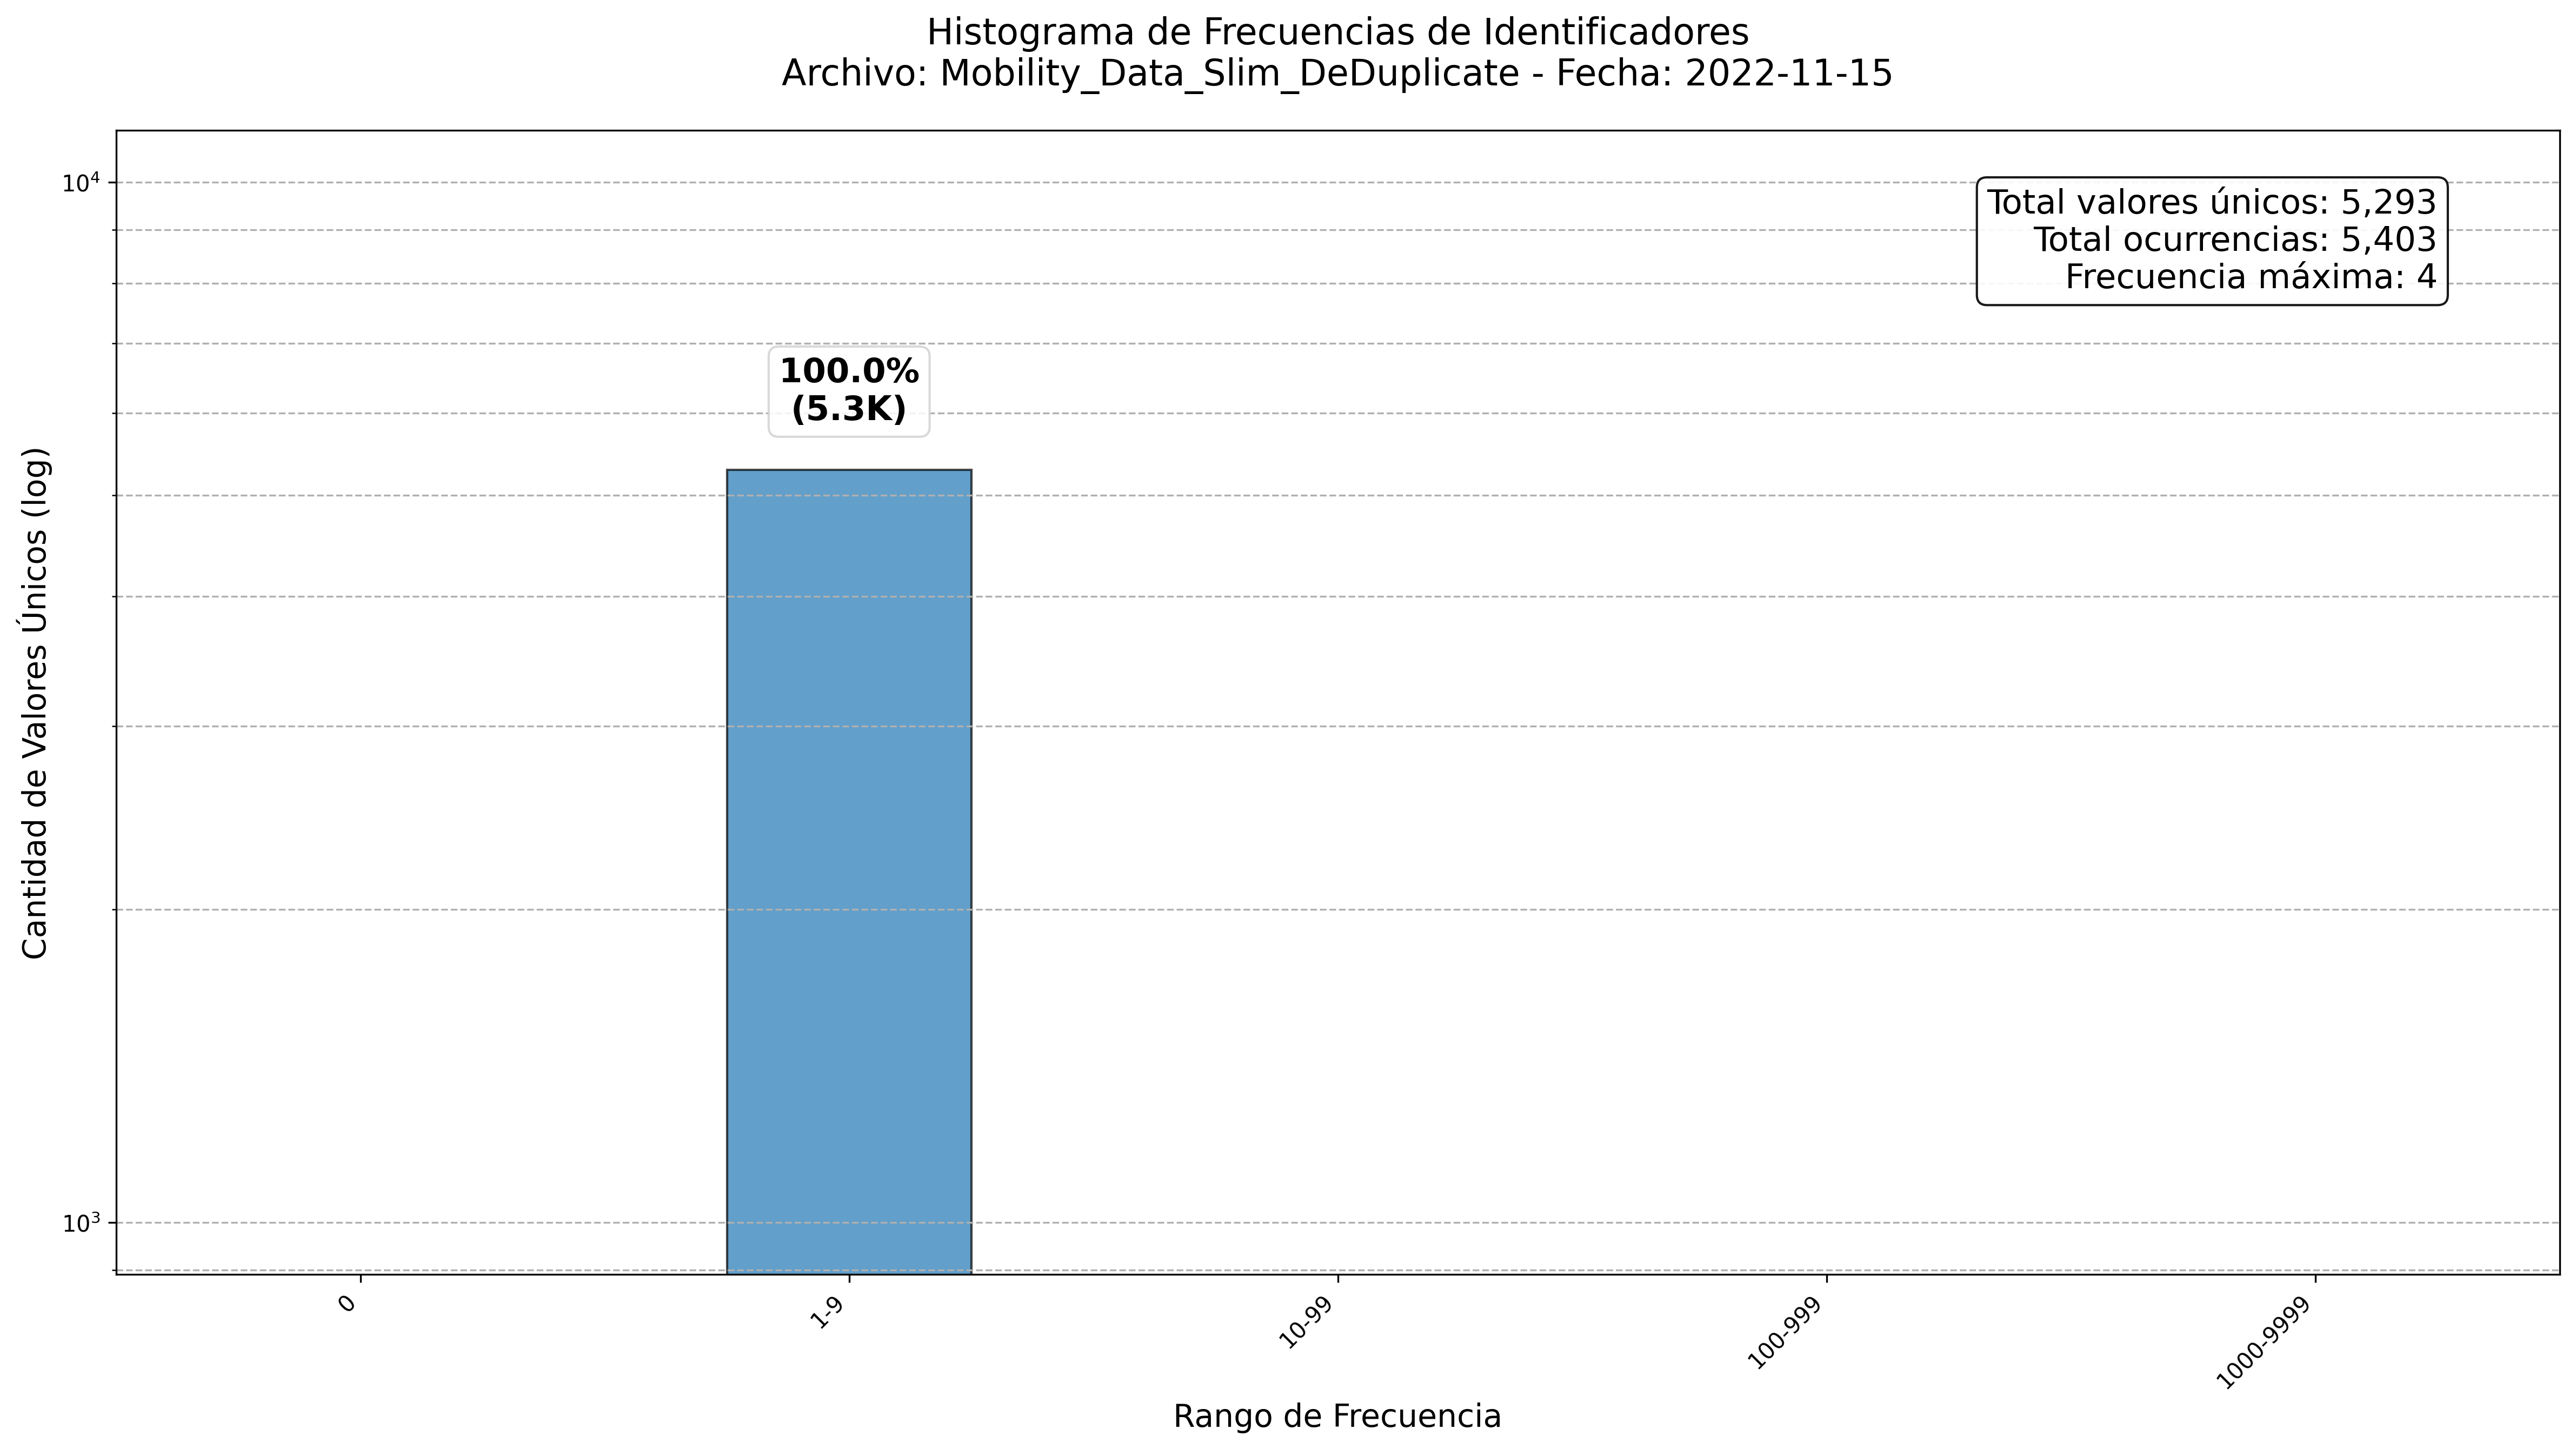
\includegraphics[width=\linewidth]{img/daily_histograms/histograma_identifier_Mobility_Data_Slim_DeDuplicate_2022-11-15.png}
        \caption{Histograma del 15/Nov/2022}
        \label{fig:sub10}
    \end{subfigure}
    \caption{Comparación de distribución de individuos por día.}
    \label{fig:histogramas_daily}
\end{figure}

De la figura anterior se puede observar que la distribución de individuos por día es bastante similar a la distribución vista en la Figura \ref{fig:identifier_histogram_deduplicate}, donde se observa que la mayoría de los individuos tienen una frecuncia de aparición baja. Además se puede ver que los primros seis días hay en promedio \textbf{1,400,000} de individuos, mientras que los últimos cuatro días este valor va disminuyendo hasta llegar a \textbf{5,293} individuos el día 15 de noviembre. Esto puede ser un indicativo de que la recolección de datos no fue constante a lo largo del tiempo, lo que podría deberse a diversos factores como problemas técnicos o cambios en el comportamiento de los individuos.